\section{Validierung}
Um die Forschungsfragen zu beantworten, haben wir die gesammelten Immobiliendaten auf Verwertbarkeit analysiert und gefiltert. Die bereinigten Inserate wurden für den Vergleich der verschiedenen Machine Learning Algorithmen verwendet. Dabei dienten der MAPE sowie der MdAPE als wichtigste Performanzkriterien. Weiter war uns wichtig, wie viele Inserate mit einer maximalen Abweichung von 10\% geschätzt werden können. Mit Hilfe von Feature Engineering und Parameter Optimierung wurde versucht, die Lernalgorithmen zu verbessern.\\
751 Inserate haben so extreme Werte, dass sie die Statistik verzerrten und so eine Aussage über die Daten erschwerten. Deshalb wurden diese Werte für die Validation ignoriert.

\subsection{Gesammelte Daten}
Insgesamt konnten 162’225 Immobilieninserate in einem Zeitraum von 5 Monaten gesammelt werden. Davon stammten die meisten vom Immoscout24 Portal, wie in Tabelle \ref{tab:crawled_data} ersichtlich.

\begin{table*}[ht]
\centering
\ra{1.3}
\begin{tabular}{@{}lrr@{}}
\toprule
Portal &  Anz. gesammelte Inserate & Anz. verwendete Inserate \\
\midrule
Immoscout24 & 94'611 & 46'226\\
Homegate & 34'115 & 19'568\\
Newhome & 32'600 & 19'011\\
Urbanhome & 2'047 & 1'040\\
\bottomrule
\end{tabular}
\caption{Auswertung der gesmmelten Daten}
\label{tab:crawled_data}
\end{table*}

Von den insgesamt 162’225 Inseraten wurden 77’608 ungültige Inserate herausgefiltert.
Dabei handelte es sich mehrheitlich um fehlerhafte Inserate oder Inserate, bei denen wichtige Kennwerte fehlten.\\
Insgesamt konnten 83’107 Wohungen und 65’430 Häuser gesammelt werden. Die restlichen Inserate waren Lagerräume oder nicht definierte Immobilien\-typen.\\
Weiter konnte für 99\% aller Inserate die Gemeinde zugeordnet, sowie für 83\% aller Inserate, mit einer vollständigen Adresse, eine Lärmbelastung berechnet werden.\\
Die meisten Inserate hatten eine Angabe über die Anzahl Zimmer und Wohnfläche, gefolgt vom Baujahr und der Anzahl an Stockwerken, falls es mehrere gab. Die Raumhöhe, die Kubatur und die Gesamtfläche einer Immobilie wurden dagegen nur selten angegeben. Abbildung \ref{fig:features} zeigt den prozentualen Anteil der fehlenden Kennwerte.

\begin{figure}[h!]
\centering
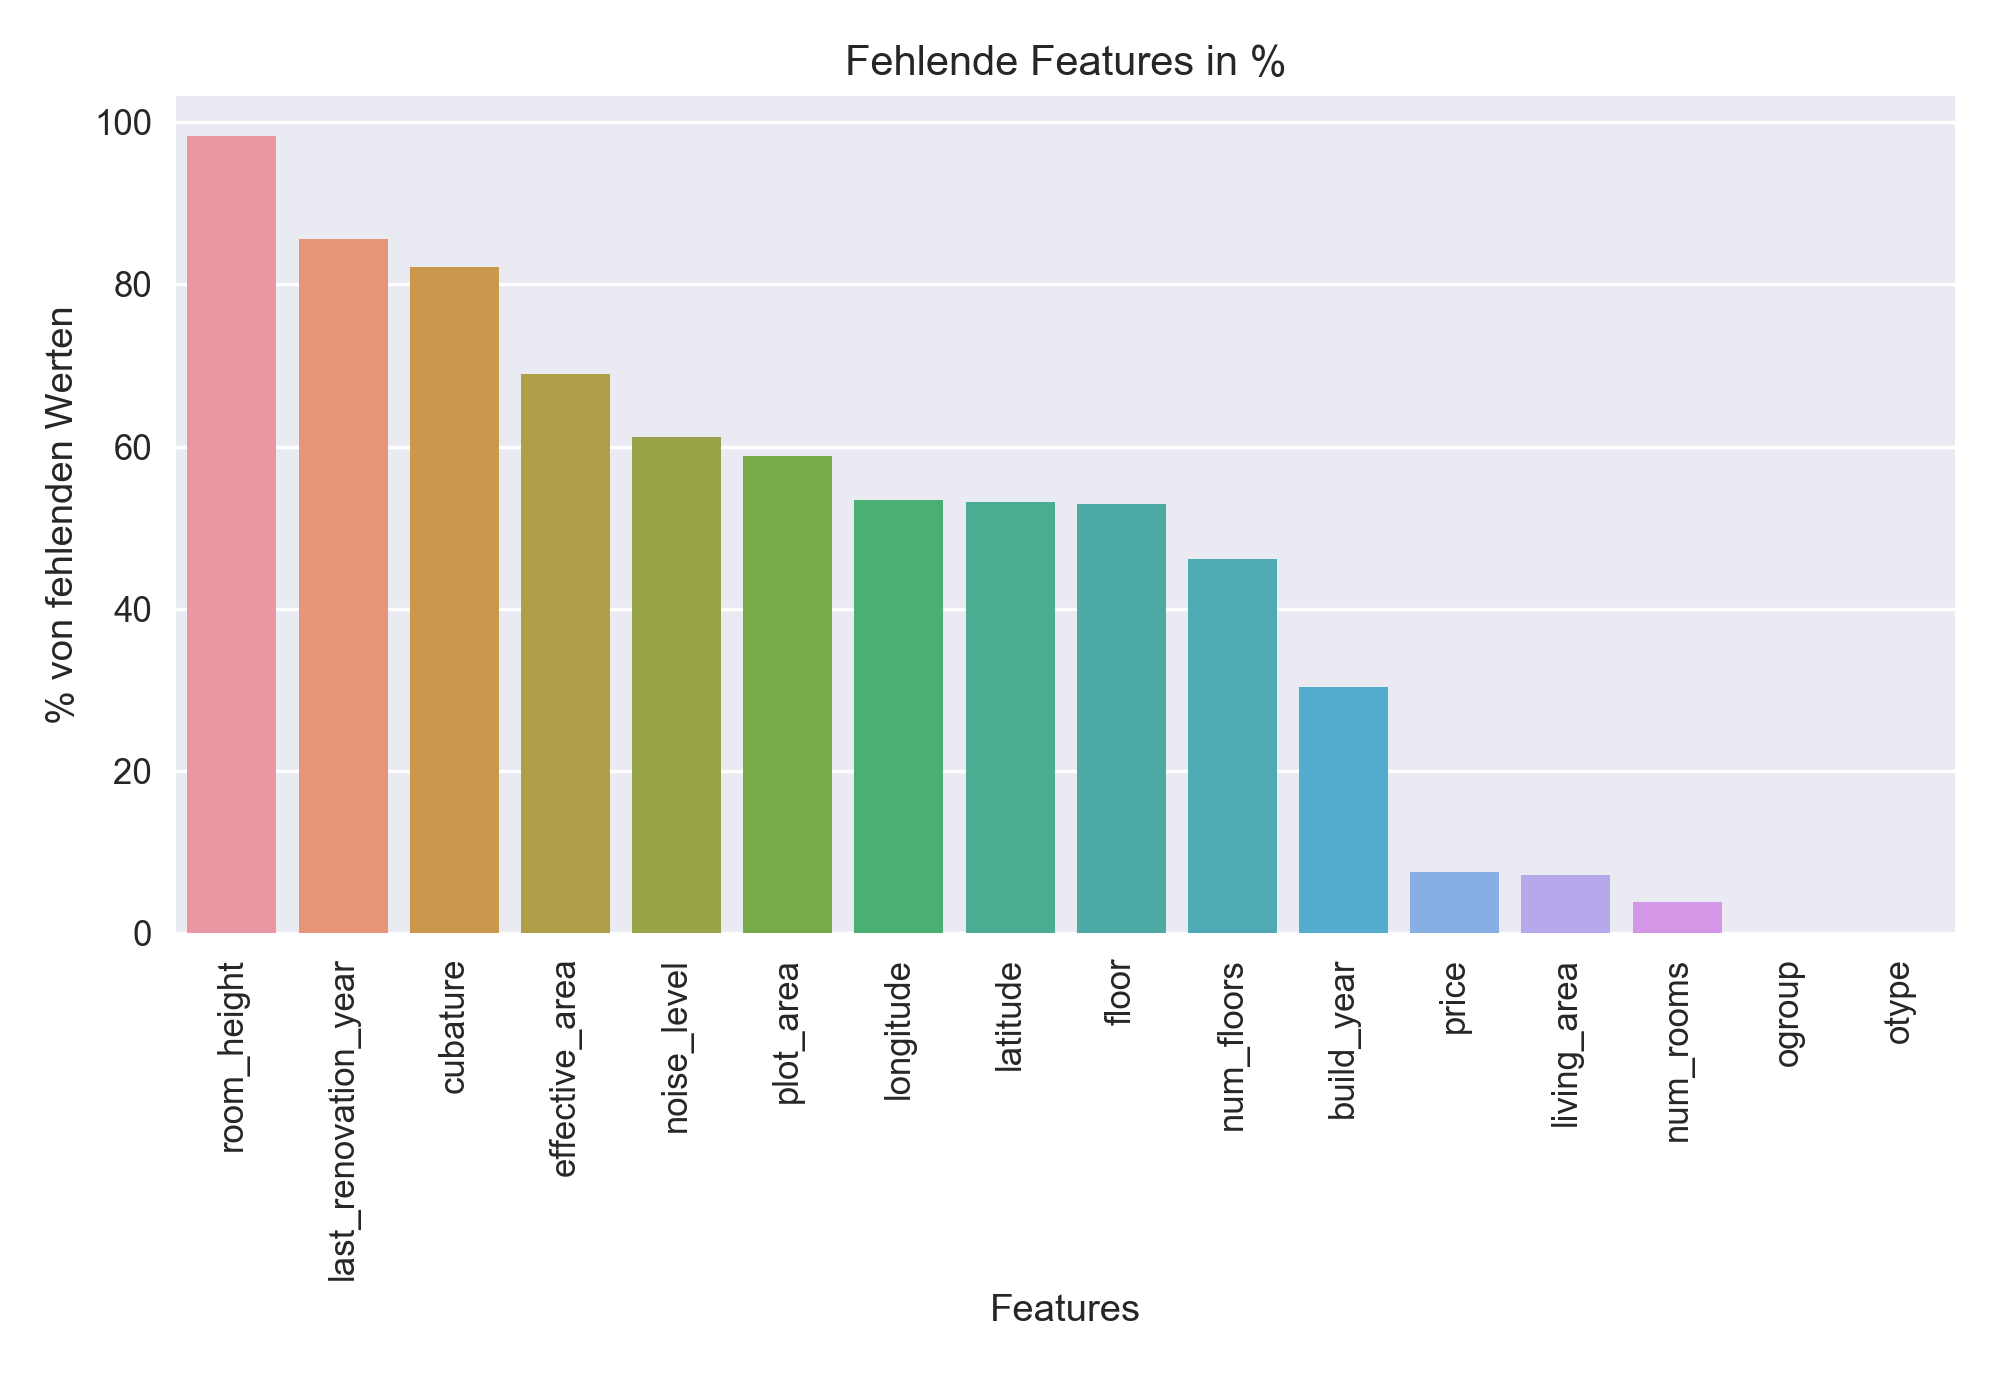
\includegraphics[width=0.9\textwidth]{images/missing_values.png}
\caption[\% Anteil der fehlenden Features]{\% Anteil der fehlenden Features}%
\label{fig:features}
\end{figure}

Die Crawler wurden nie über eine längere Zeit gesperrt. Vereinzelt kam es zu Blockierungen, die jedoch, durch das Starten neuer Proxyinstanzen, umgangen werden konnten. Der Zeitaufwand um ein Portal bei fünf gleichzeitigen Verbindungen und einer Downloaddelay von zwei Sekunden zu crawlen, lag im Schnitt bei 4 Stunden. Dementsprechend wurden in dieser Zeit etwa 100 Proxyinstanzen gestartet.\\[2ex]
%
Die Datenqualität der gesammelten Inserate war eher mässig, viele Features konnten nicht für das Machine Learning verwendet werden. Um dem entgegenzuwirken, wurde versucht durch Feature Engineering neue Features zu generieren.

\subsubsection{Kaufpreis}
Abbildung \ref{fig:price} zeigt die Verteilung der Kaufpreise. Abbildung \ref{fig:verteilung_price_all} beinhaltet alle Inserate wobei Abbildung \ref{fig:verteilung_price_part} nur die Inserate von 0 CHF - 3,5 Mio. CHF aufzeigt. Dabei ist ersichtlich, dass der Preis nicht normalverteilt ist. Es besteht eine positive Skenwess, was für eine lineare Regression nicht optimal ist.\\
Die Mehrheit der Preise befindet sich zwischen 250'000 CHF und 1.2 Mio. CHF. Daneben kommen mehrheitlich teurere Immobilien vor. Tabelle \ref{tab:price} zeigt die beschreibenden statistischen Werte des Kaufpreises vor dem Feature Engineering. Es ist zu sehen, dass die Standardabweichung von Wohnungen fast halb so gross ist, wie die der Häuser. Das liegt unter anderem daran, dass unsere gesammelten Wohnungspreise kein grosses Preisspektrum besitzen. Zum Vergleich werden im Kapitel Feature Engineering die beschreibenden statistischen Werte des Preises nach der Outlier Detection angezeigt.

\begin{figure}[ht]
\begin{subfigure}{.5\textwidth}
  \centering
  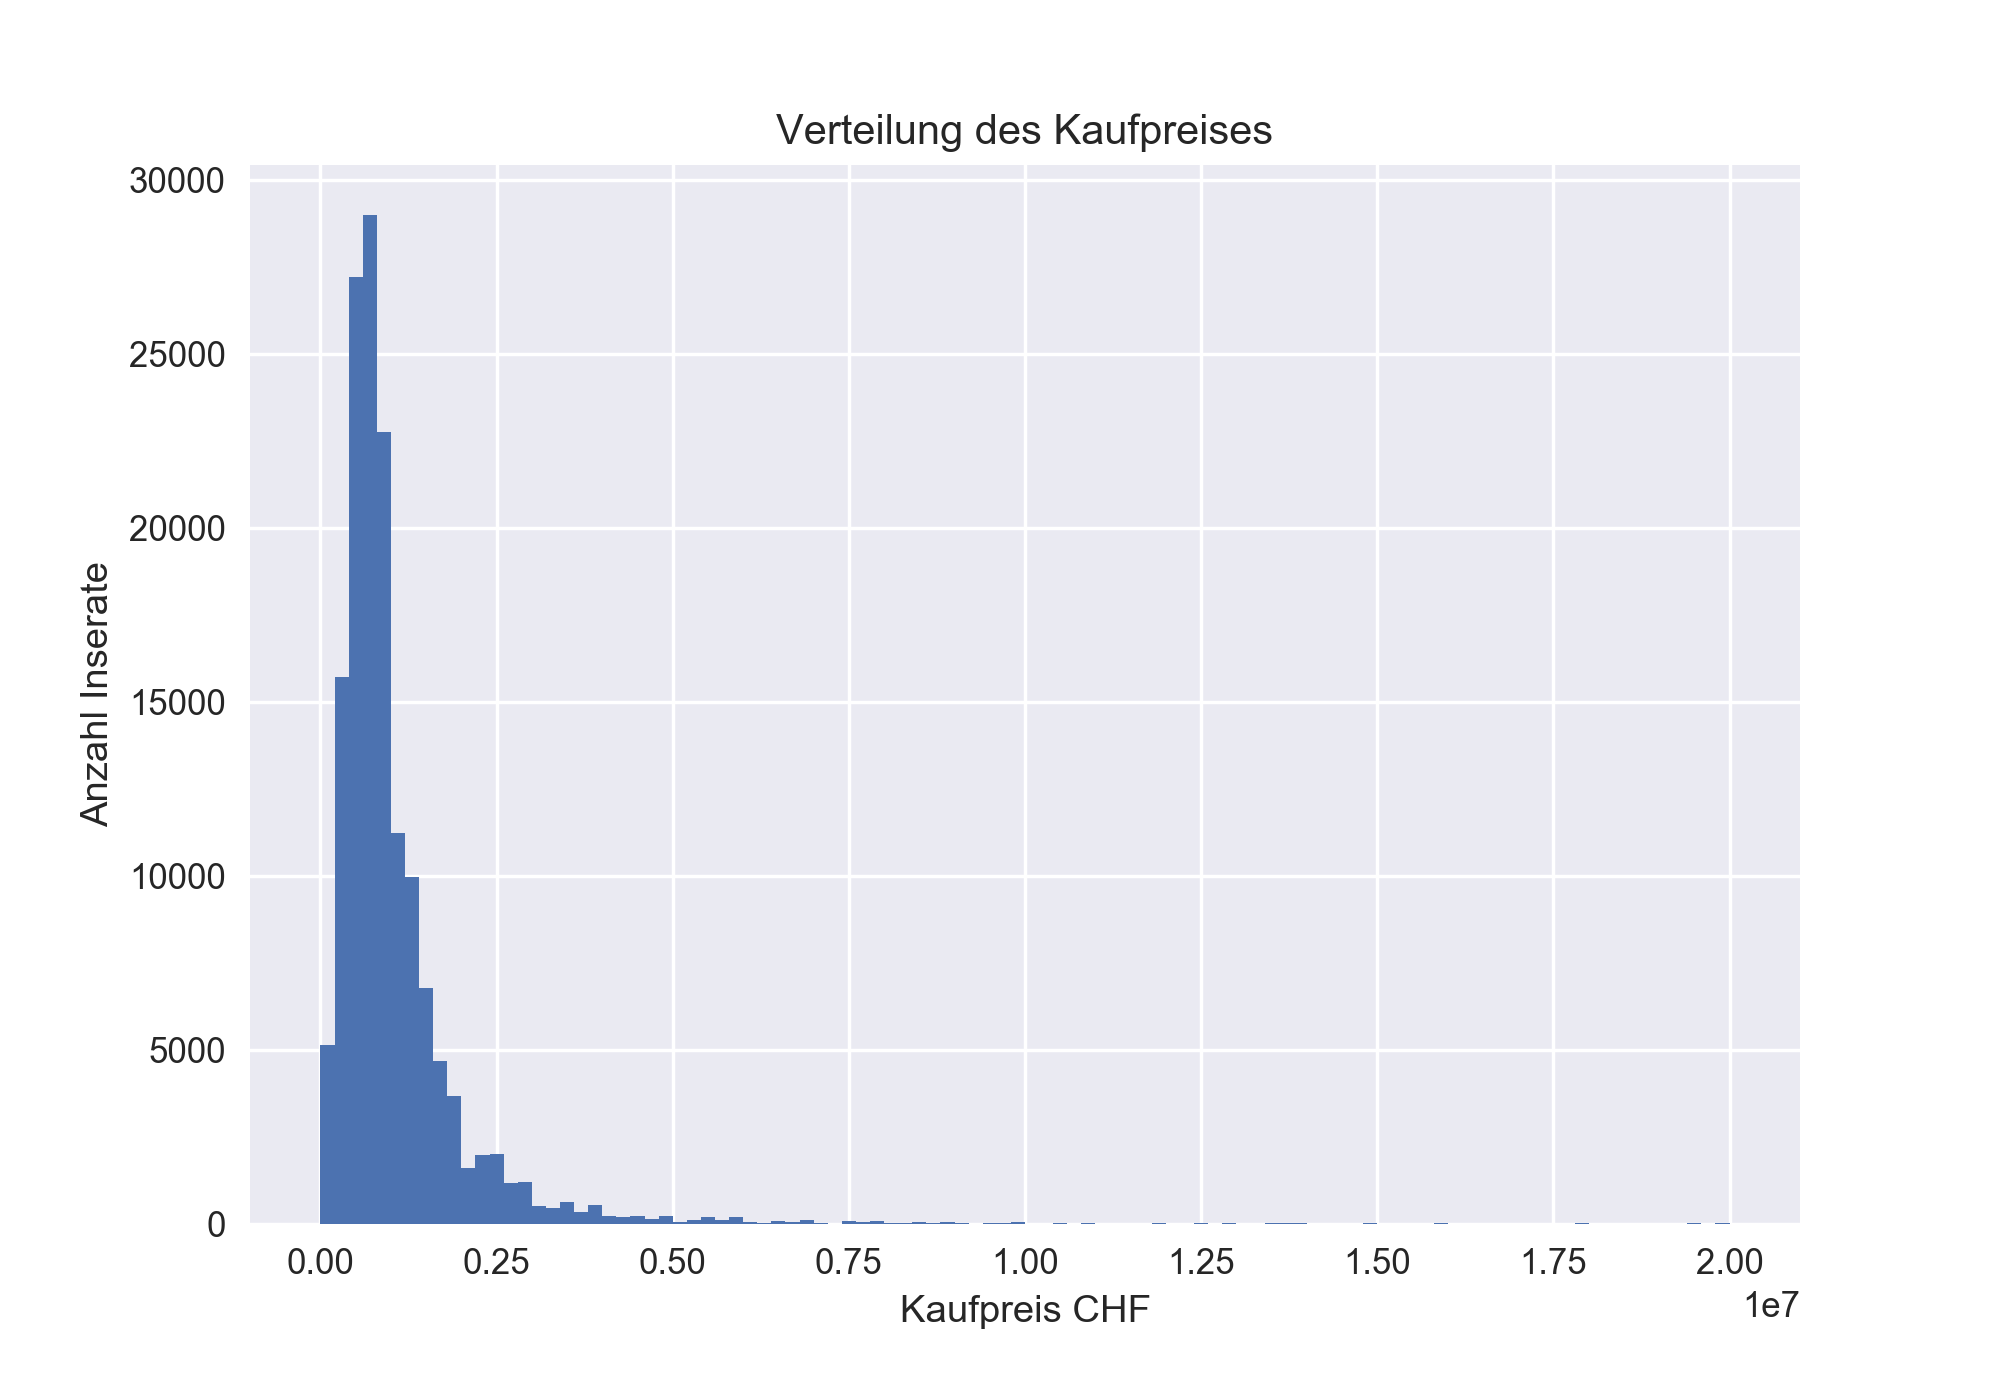
\includegraphics[width=\linewidth]{images/bar_des_kauf_preises.png}
  \caption[Verteilung des Preises mit allen Daten]{Verteilung des Preises mit allen Daten\\}
  \label{fig:verteilung_price_all}
\end{subfigure}
\begin{subfigure}{.5\textwidth}
  \centering
  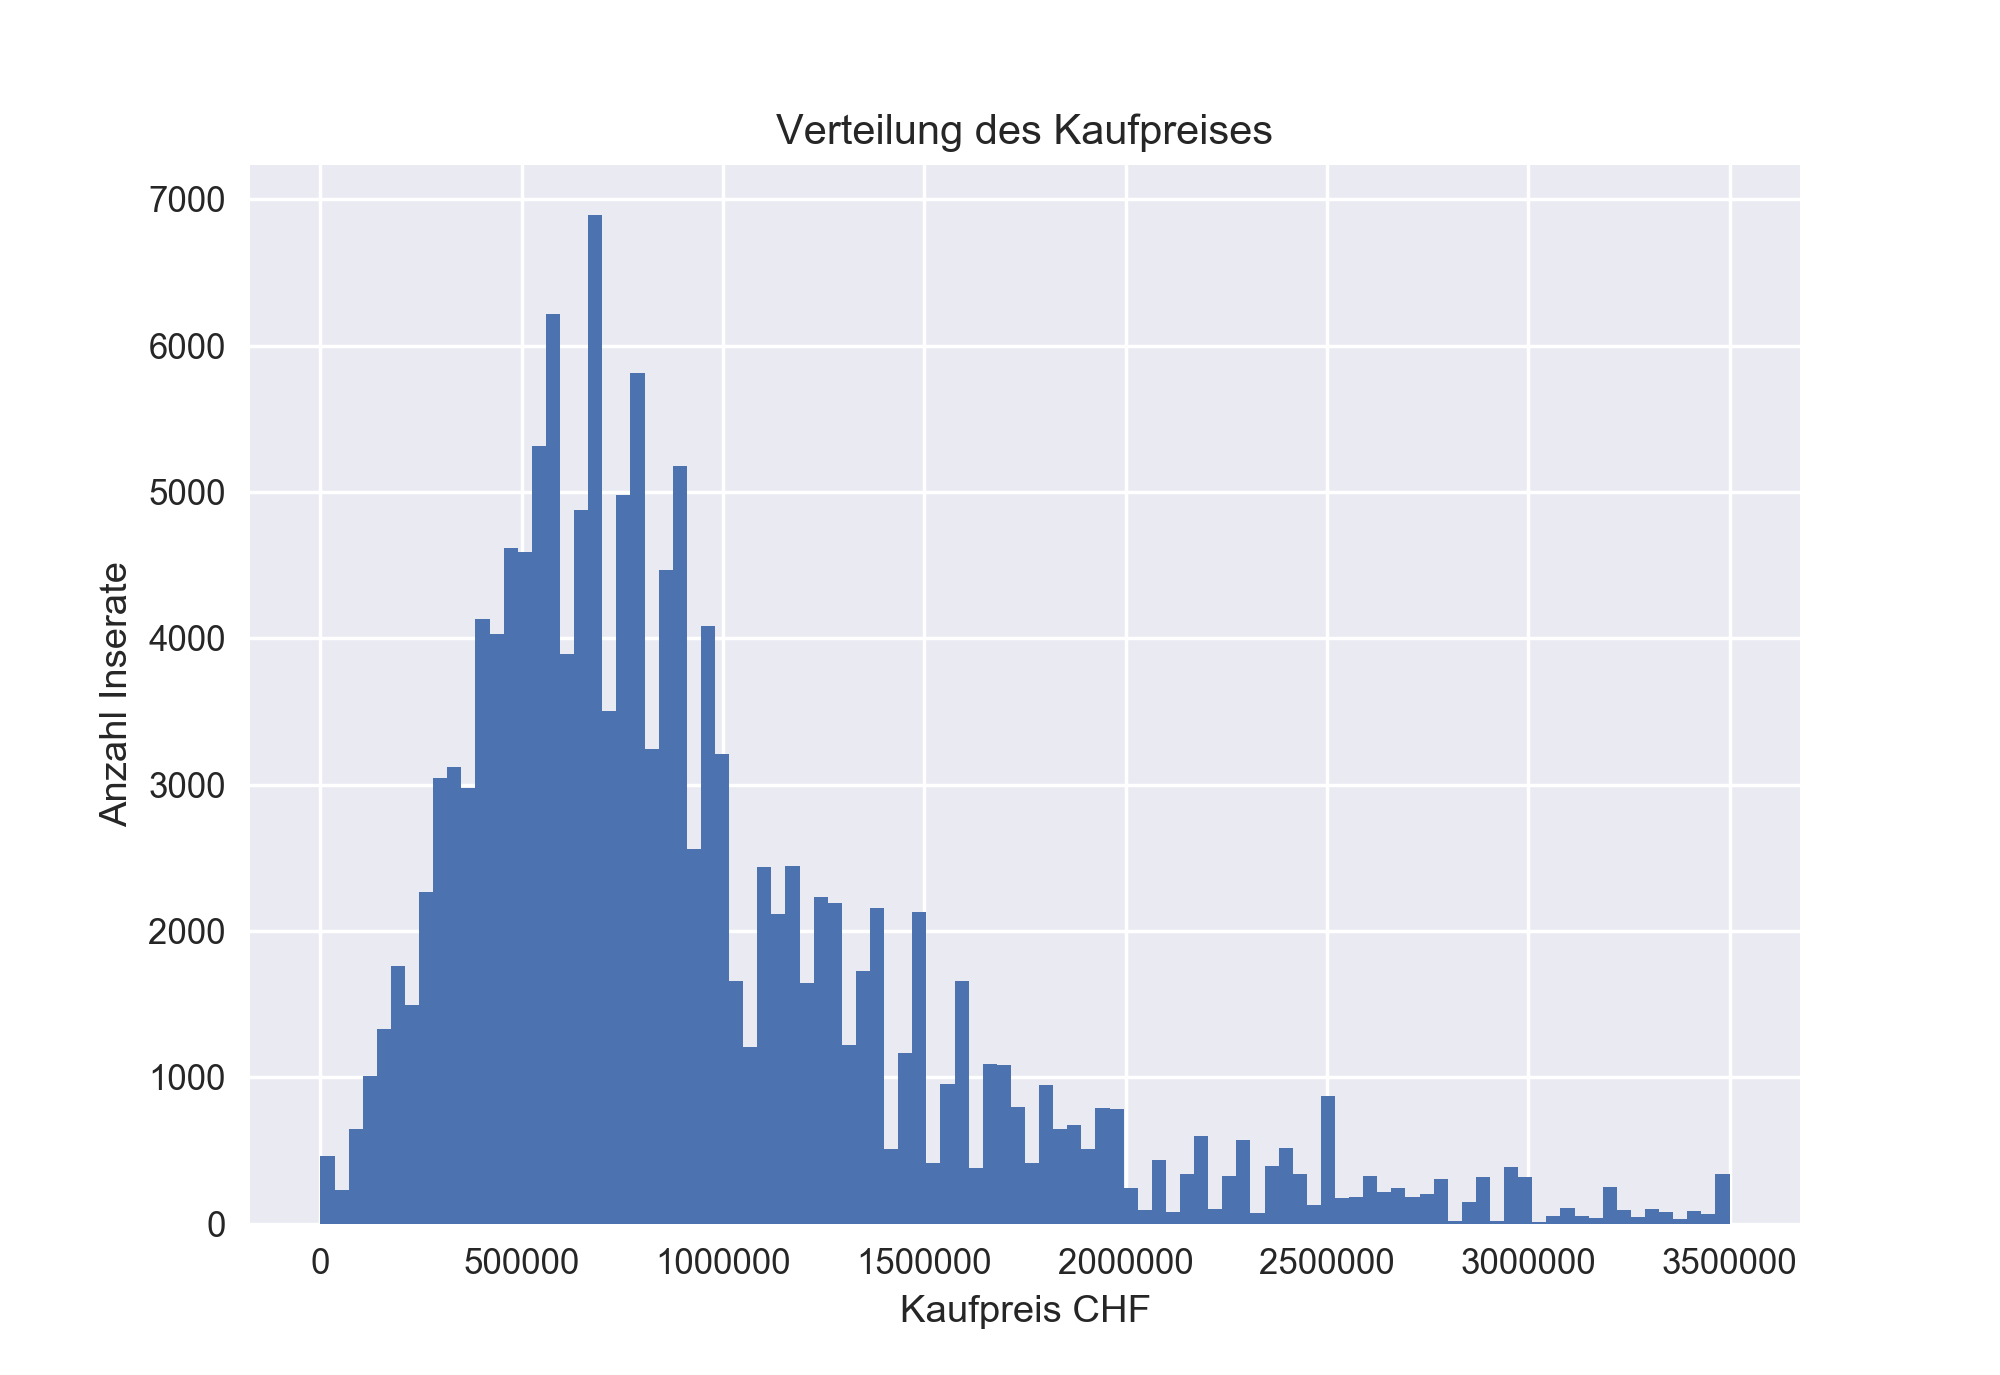
\includegraphics[width=\linewidth]{images/bar_des_kauf_preises_cut.png}
  \caption[Verteilung des Preises von 0 CHF - 2.5 Mio CHF]{Verteilung des Preises von 0 CHF - 2.5 Mio CHF}
  \label{fig:verteilung_price_part}
\end{subfigure}
\caption[Verteilung des Kaufpreises]{Verteilung des Kaufpreises}
\label{fig:price}
\end{figure}

\begin{table*}[ht]
\centering
\ra{1.3}
\resizebox{\textwidth}{!}{
\begin{tabular}{@{}lrrrrr@{}}
\toprule
Objektart & Min & Max & Durchschnitt & Median & Standardabweichung\\
\midrule
Wohnung & 10 & 20'000'000 & 891’479 & 690’000 & 786’047\\
Haus & 10 & 20'000'000 & 1'281'735 & 920'000 & 1'309'085\\
Wohnung \& Haus & 10 & 20’000'000 & 1’059’503 & 790’000 & 1’066’372\\
\bottomrule
\end{tabular}}
\caption{Statistische Werte des Kaufpreises}
\label{tab:price}
\end{table*}

\subsubsection{Numerische Features}
Bis auf die Lärmbelastung wurden alle numerischen Features von den Immobilienportalen gesammelt.\\
Abbildung \ref{fig:num_features} zeigt einen Teil dieser Features in Verbindung zum Kaufpreis. Dabei ist ersichtlich, dass die Wohnfläche, Kubatur und Anzahl Zimmer eine linear ähnliche Abhängigkeit besitzen. Die restlichen Features beistzen keine direkte Korrelation zum Preis.

\begin{figure}[h]
\centering
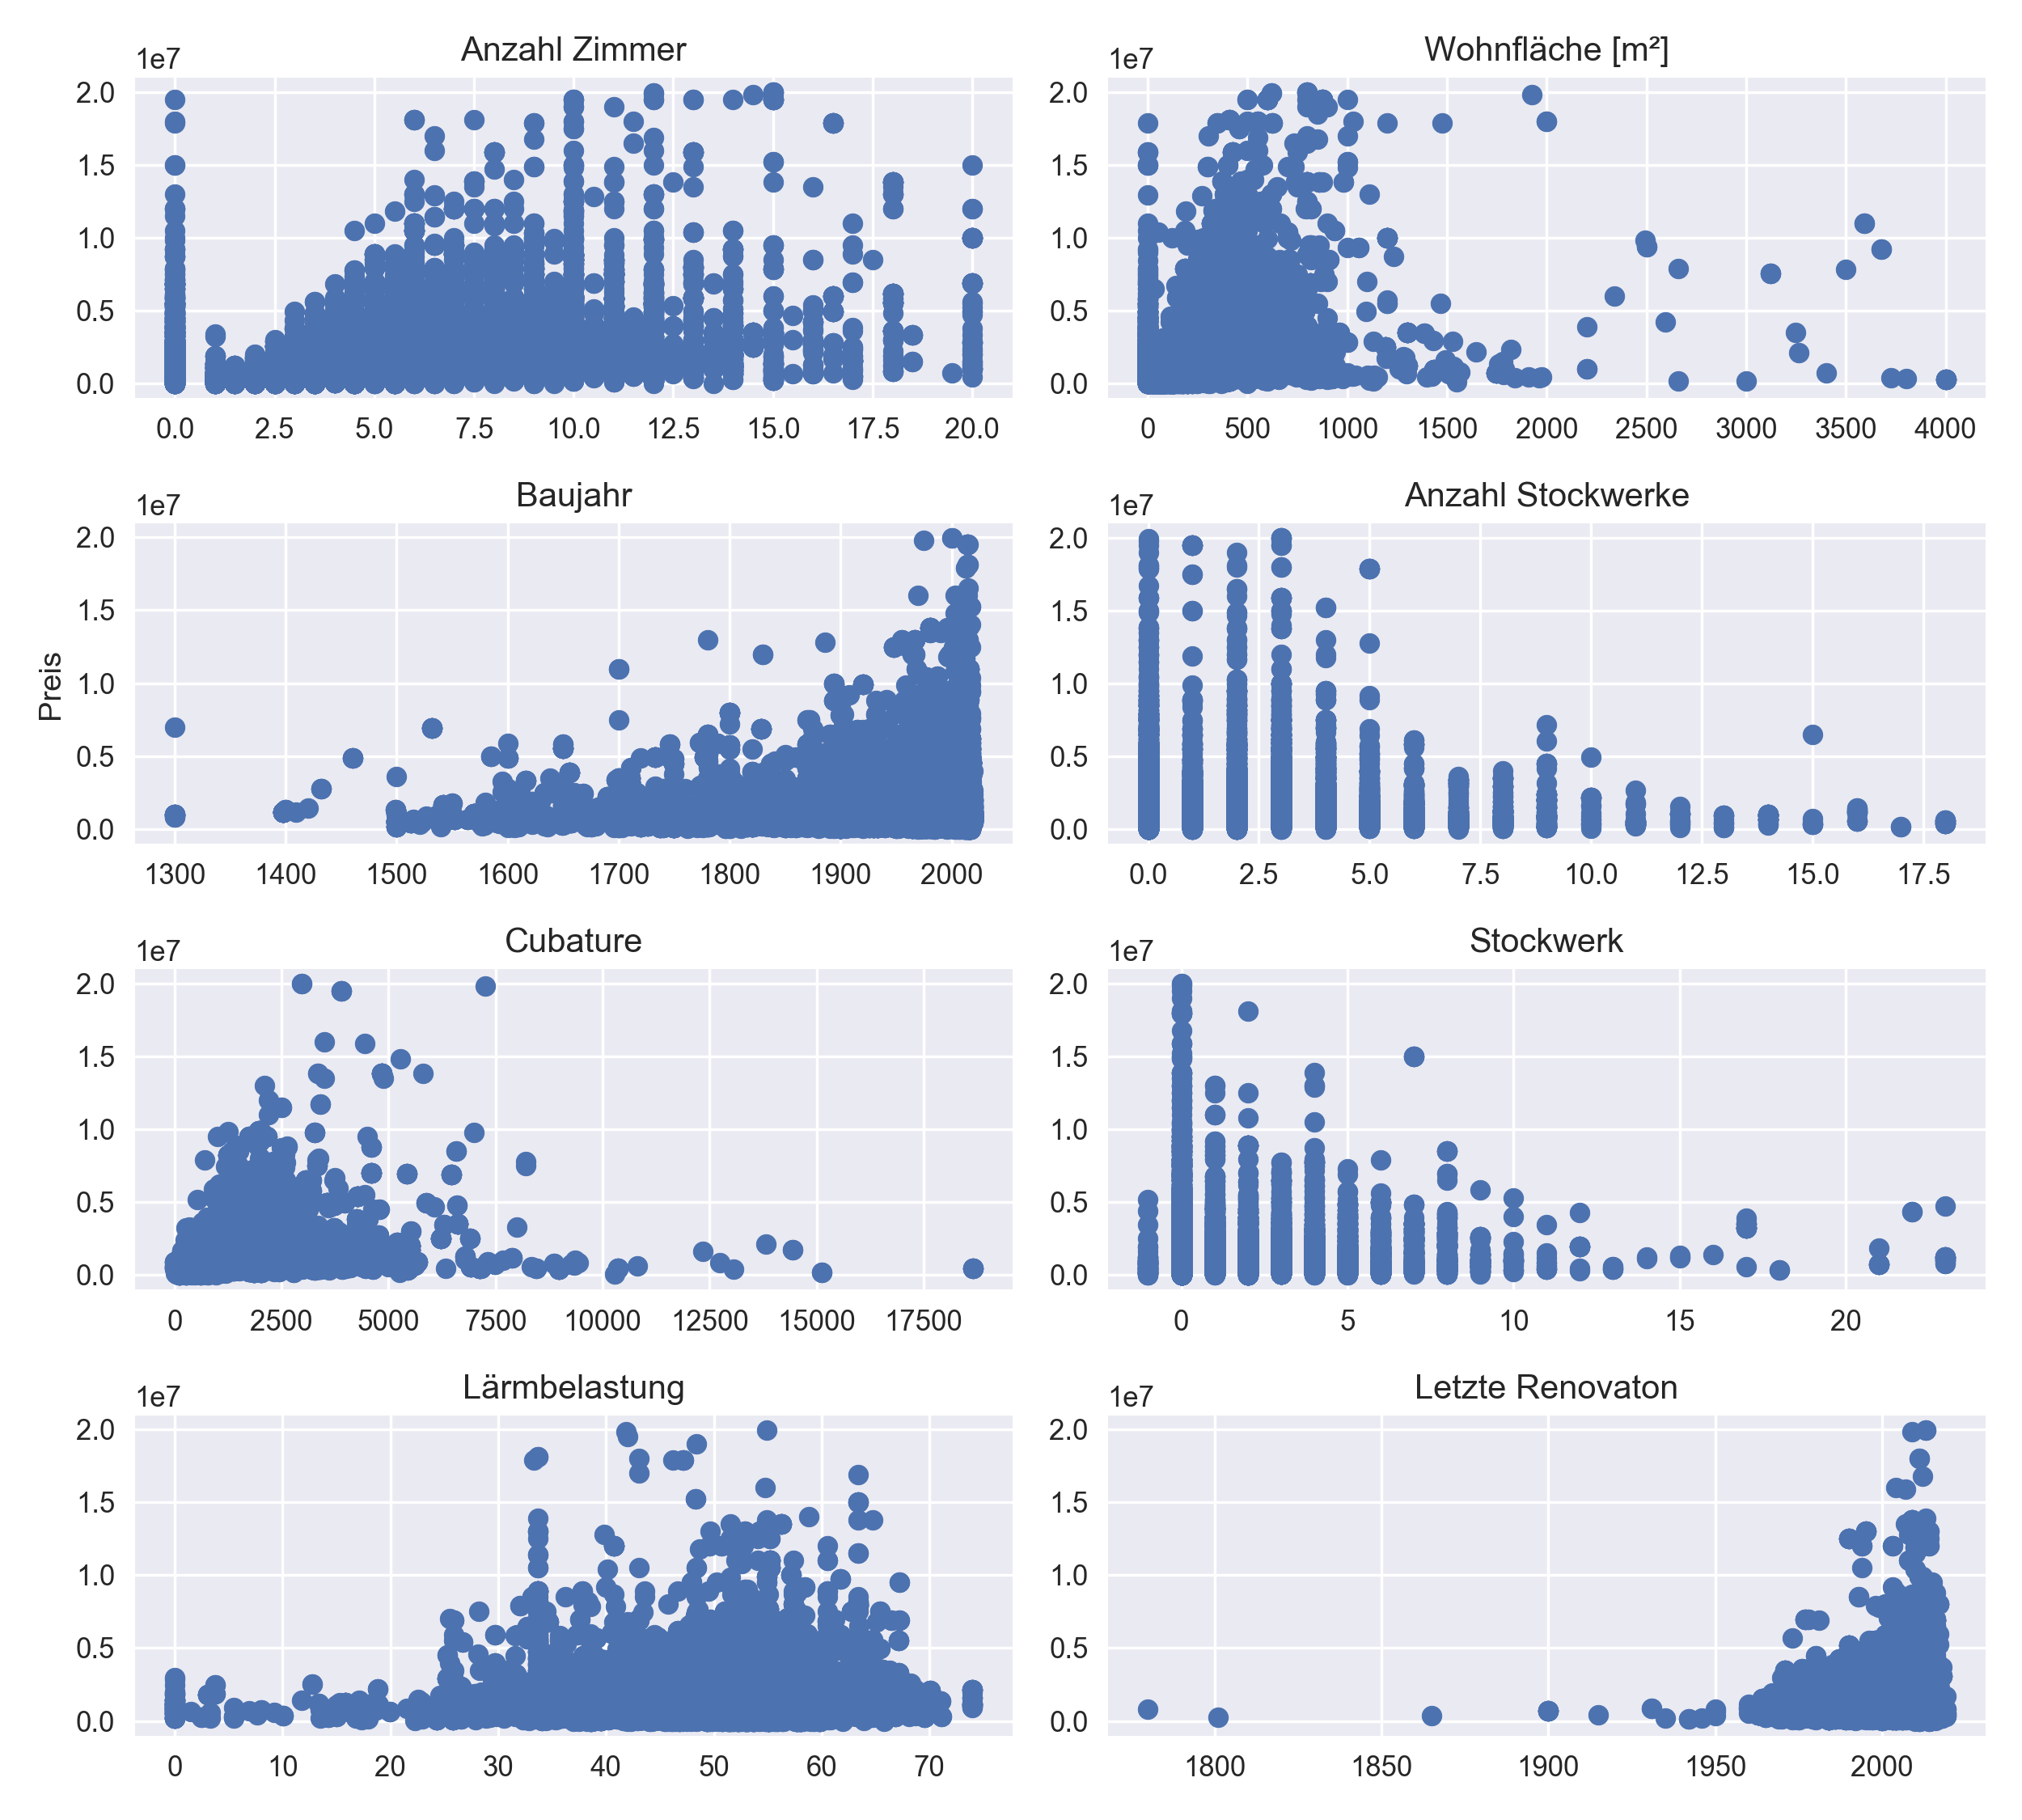
\includegraphics[width=\textwidth]{images/Vergleich_zum_preis.png}
\caption[Numerische Features im Vergleich zum Preis]{Numerische Features im Vergleich zum Preis}%
\label{fig:num_features}
\end{figure}

Tabelle \ref{tab:num_features} zeigt die statistischen Werte für die numerischen Features. Die gesammelten Kennwerte sehen plausibel aus und decken sich zum Teil mit den Daten vom Bundesamt für Statistik\footnote{https://www.bfs.admin.ch/bfs/de/home/statistiken/bau-wohnungswesen.html}. Auffallend ist, dass der Durchschnitt und der Median bei vielen Features sehr nahe beieinander liegen. Somit gleicht die Verteilung einer Normalverteilung.

\begin{table*}[h]
\centering
\ra{1.3}
\resizebox{\textwidth}{!}{
\begin{tabular}{@{}lrrrrr@{}}
\toprule
 & Min & Max & Durchschnitt & Median & Standardabweichung\\
\midrule
Anz. Zimmer & 0& 20 & 4.84 & 4.5 & 1.9\\
Fläche & 0 & 4’000 & 143.08 & 130 & 101.924\\
Baujahr & 1300 & 2019 & 1988 & 2006 & 51.52\\
Anz. Stockwerke & 0 & 18 & 1.8 & 2 & 1.747\\
Kubatur & 1 & 18649 & 1059.74 & 867 & 838.419\\
Stockwerk & -1 & 23 & 1.25 & 1 & 1.57\\
Lärmbelastung & 0 & 73.99 & 48.8 & 49.35 & 6.85\\
Letzte Renovation & 1780 & 2019 & 2009 & 2012 & 9.09\\
\bottomrule
\end{tabular}}
\caption{Statistische Werte der numerischen Features}
\label{tab:num_features}
\end{table*}

Abbildung \ref{fig:heatmap} zeigt eine Heatmap der einzelnen Features. Diese zeigt auf, welche Features  untereinander korrelieren. Der Kaufpreis hat die höchste Korrelationen mit der Wohnfläche und der Anzahl Zimmer. Weniger starke Korrelationen besitzt er mit dem Baujahr sowie Stockwerk.

\begin{figure}[h!]
\centering
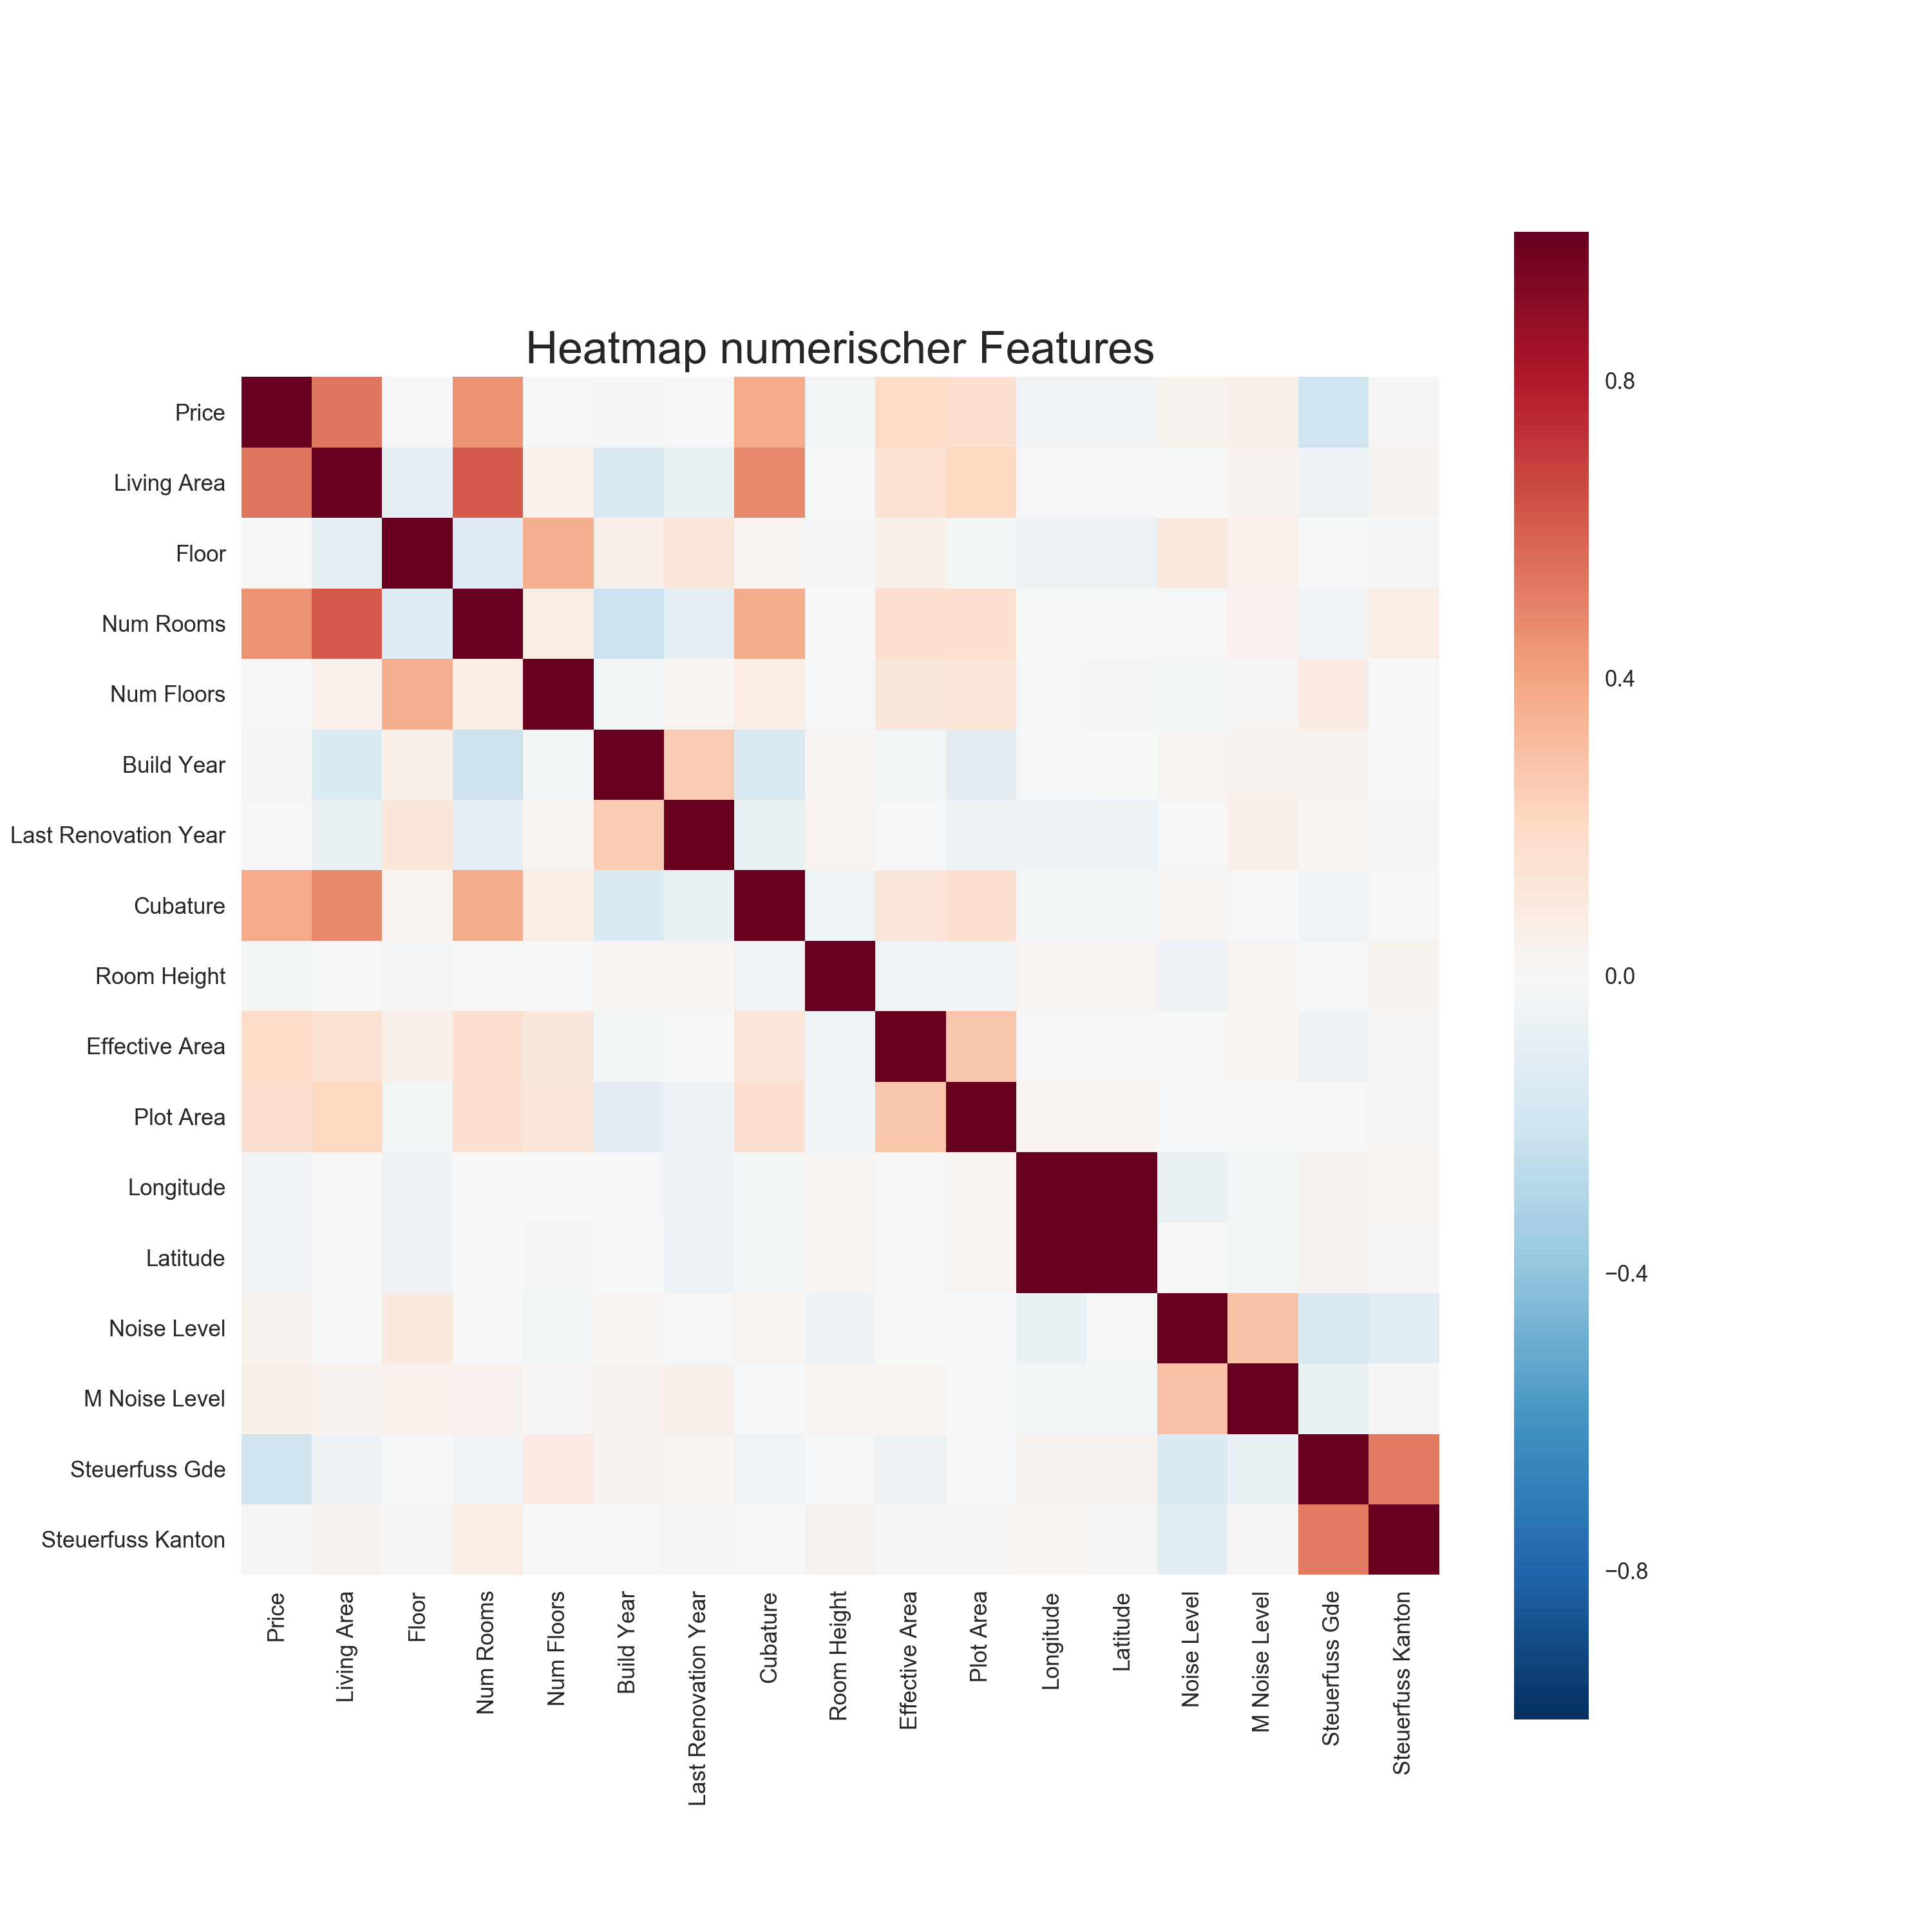
\includegraphics[width=0.9\textwidth]{images/Heatmap_numerical.png}
\caption[Heatmap der numerischen Features]{Heatmap der numerischen Features}
\label{fig:heatmap}
\end{figure}

% TODO newpage
\newpage
\subsubsection{Kategorische Features}
Bei den kategorischen Features handelte es sich vor allem um ortsbezogene Features vom BFS. Viele davon beschrieben die Region, indem sich die Immobilie befand.\\
Insgesamt wurden 35 kategorische Features verwendet. Eine Analyse der ortsbezogenen Features mit dem Kaufpreis ergab keine unerwarteten Ergebnisse. So zeigt Abbildung \ref{fig:cantons}, dass der Kanton Genf die teuersten Immobilien in der Schweiz besitzt, gefolgt vom Kanton Zug. Auch ist ersichtlich, dass städtische Immobilien im Schnitt teurer sind als auf dem Land. Anders gesagt, je urbaner die Region, desto teurer der Immobilienpreis. Diverse weitere Vergleiche befinden sich in Anhang \ref{daten_analys}.\\[2ex]
\begin{figure}[ht]
\centering
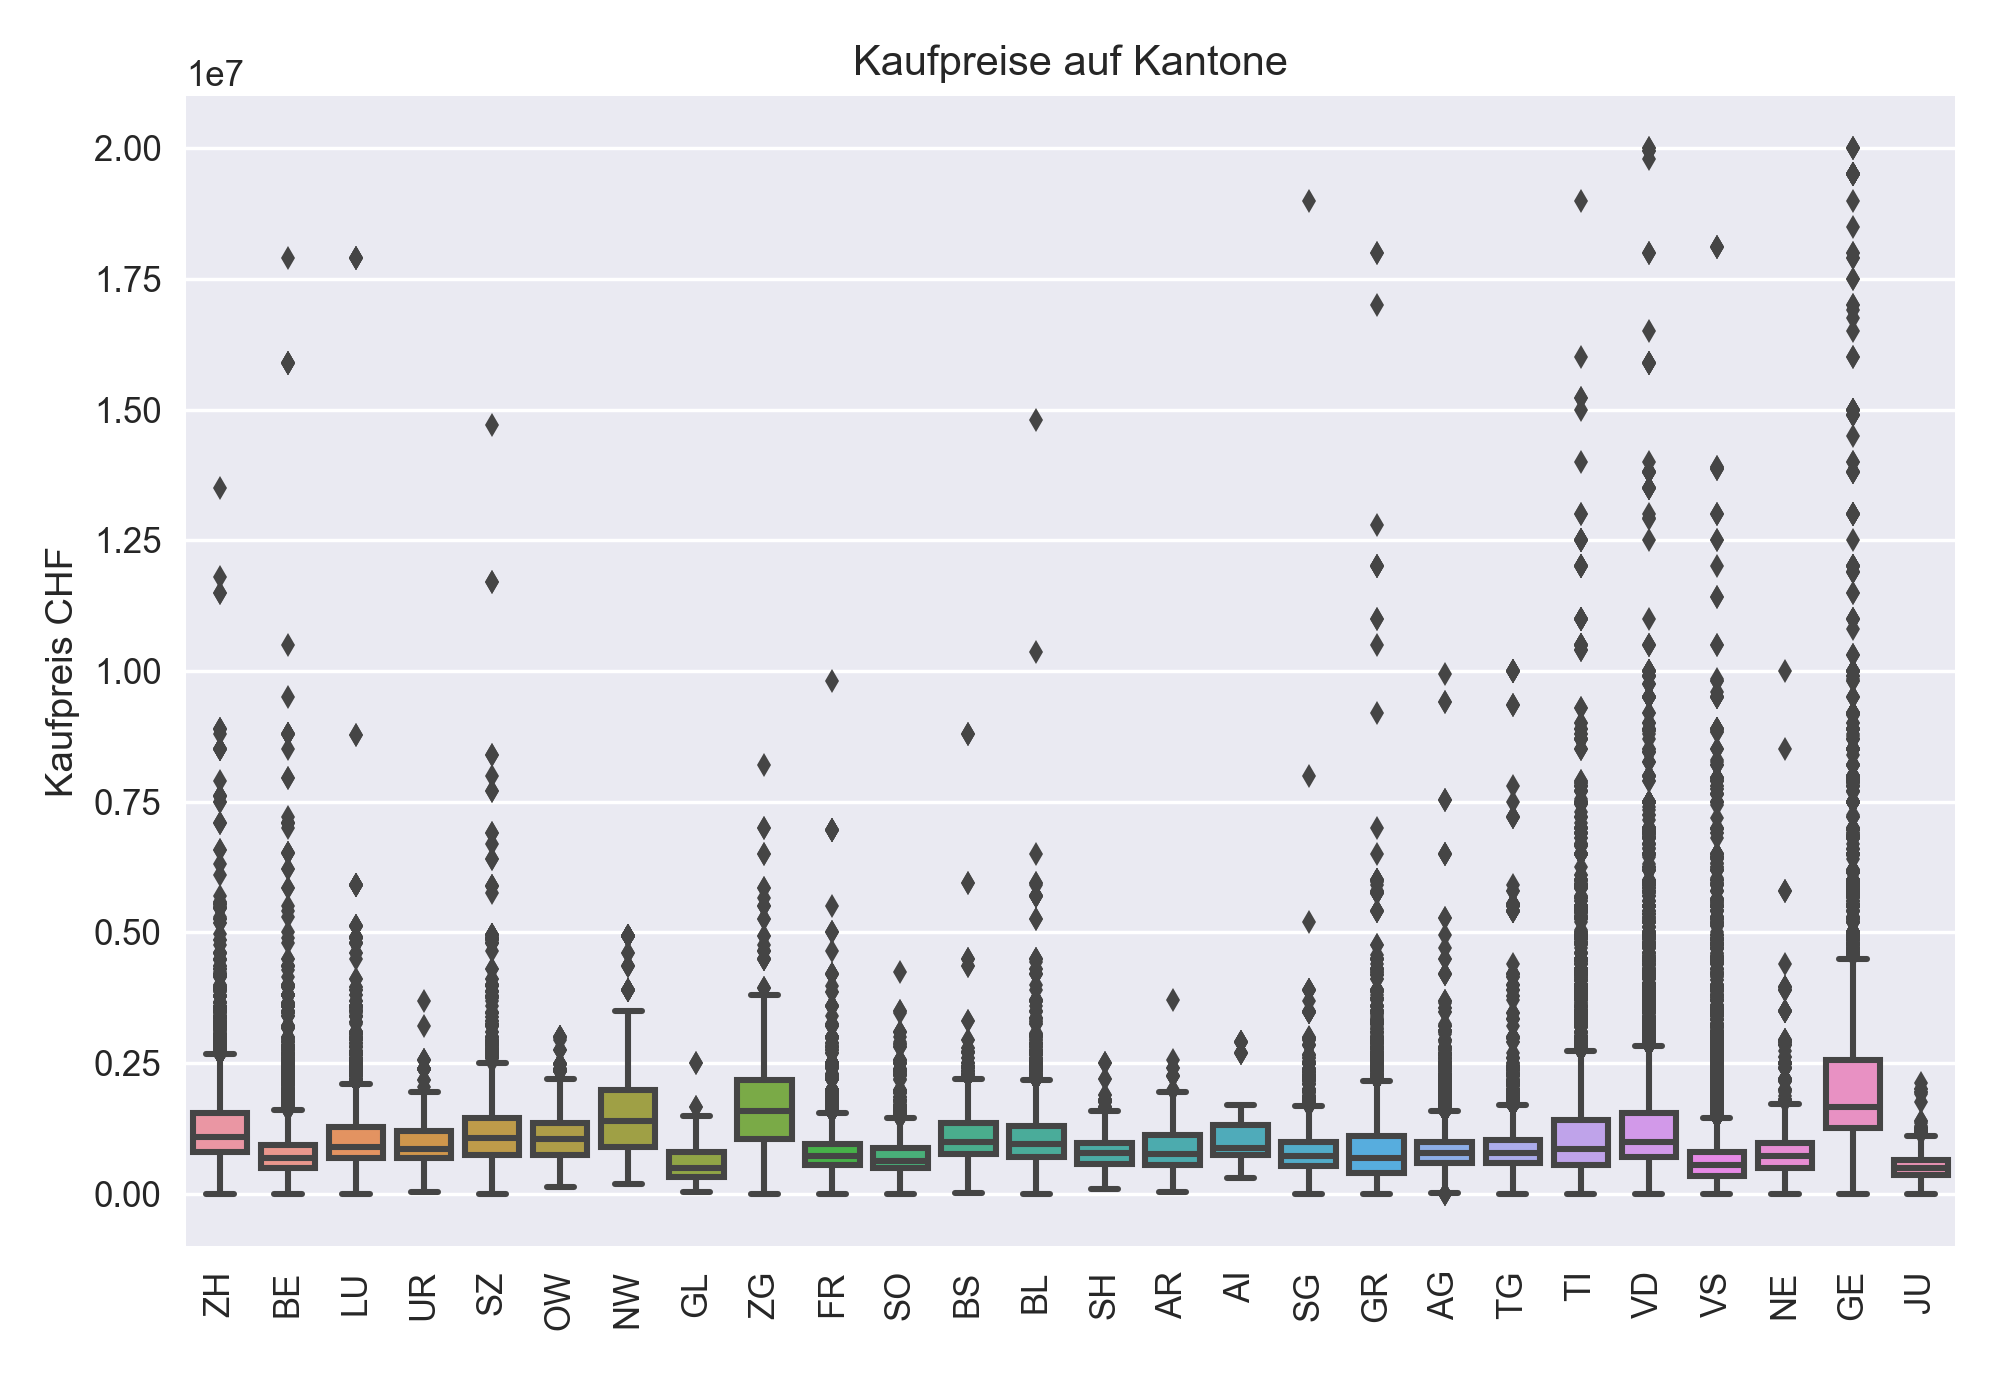
\includegraphics[width=\textwidth]{images/boxPlot_cantons.png}
\caption[Kaufpreis auf Kantonte aufgeteilt]{Kaufpreis auf Kantonte aufgeteilt}%
\label{fig:cantons}
\end{figure}

\textbf{Beschreibung / Merkmale}\\
Neben den ortsbezogenen Daten, analysierten wir die Beschreibung und die Merkmale der Inserate, um verschiedene Tags zuordnen zu können. Die 50 häufigsten vorkommenden Tags, die in unserem Datensatz vorkamen, werden in Abbildung \ref{fig:tags} gezeigt. Die verwendeten Tags beschreiben vor allem die Innen- und Ausseneinrichtung einer Immobile.
%
\begin{figure}[ht]
\centering
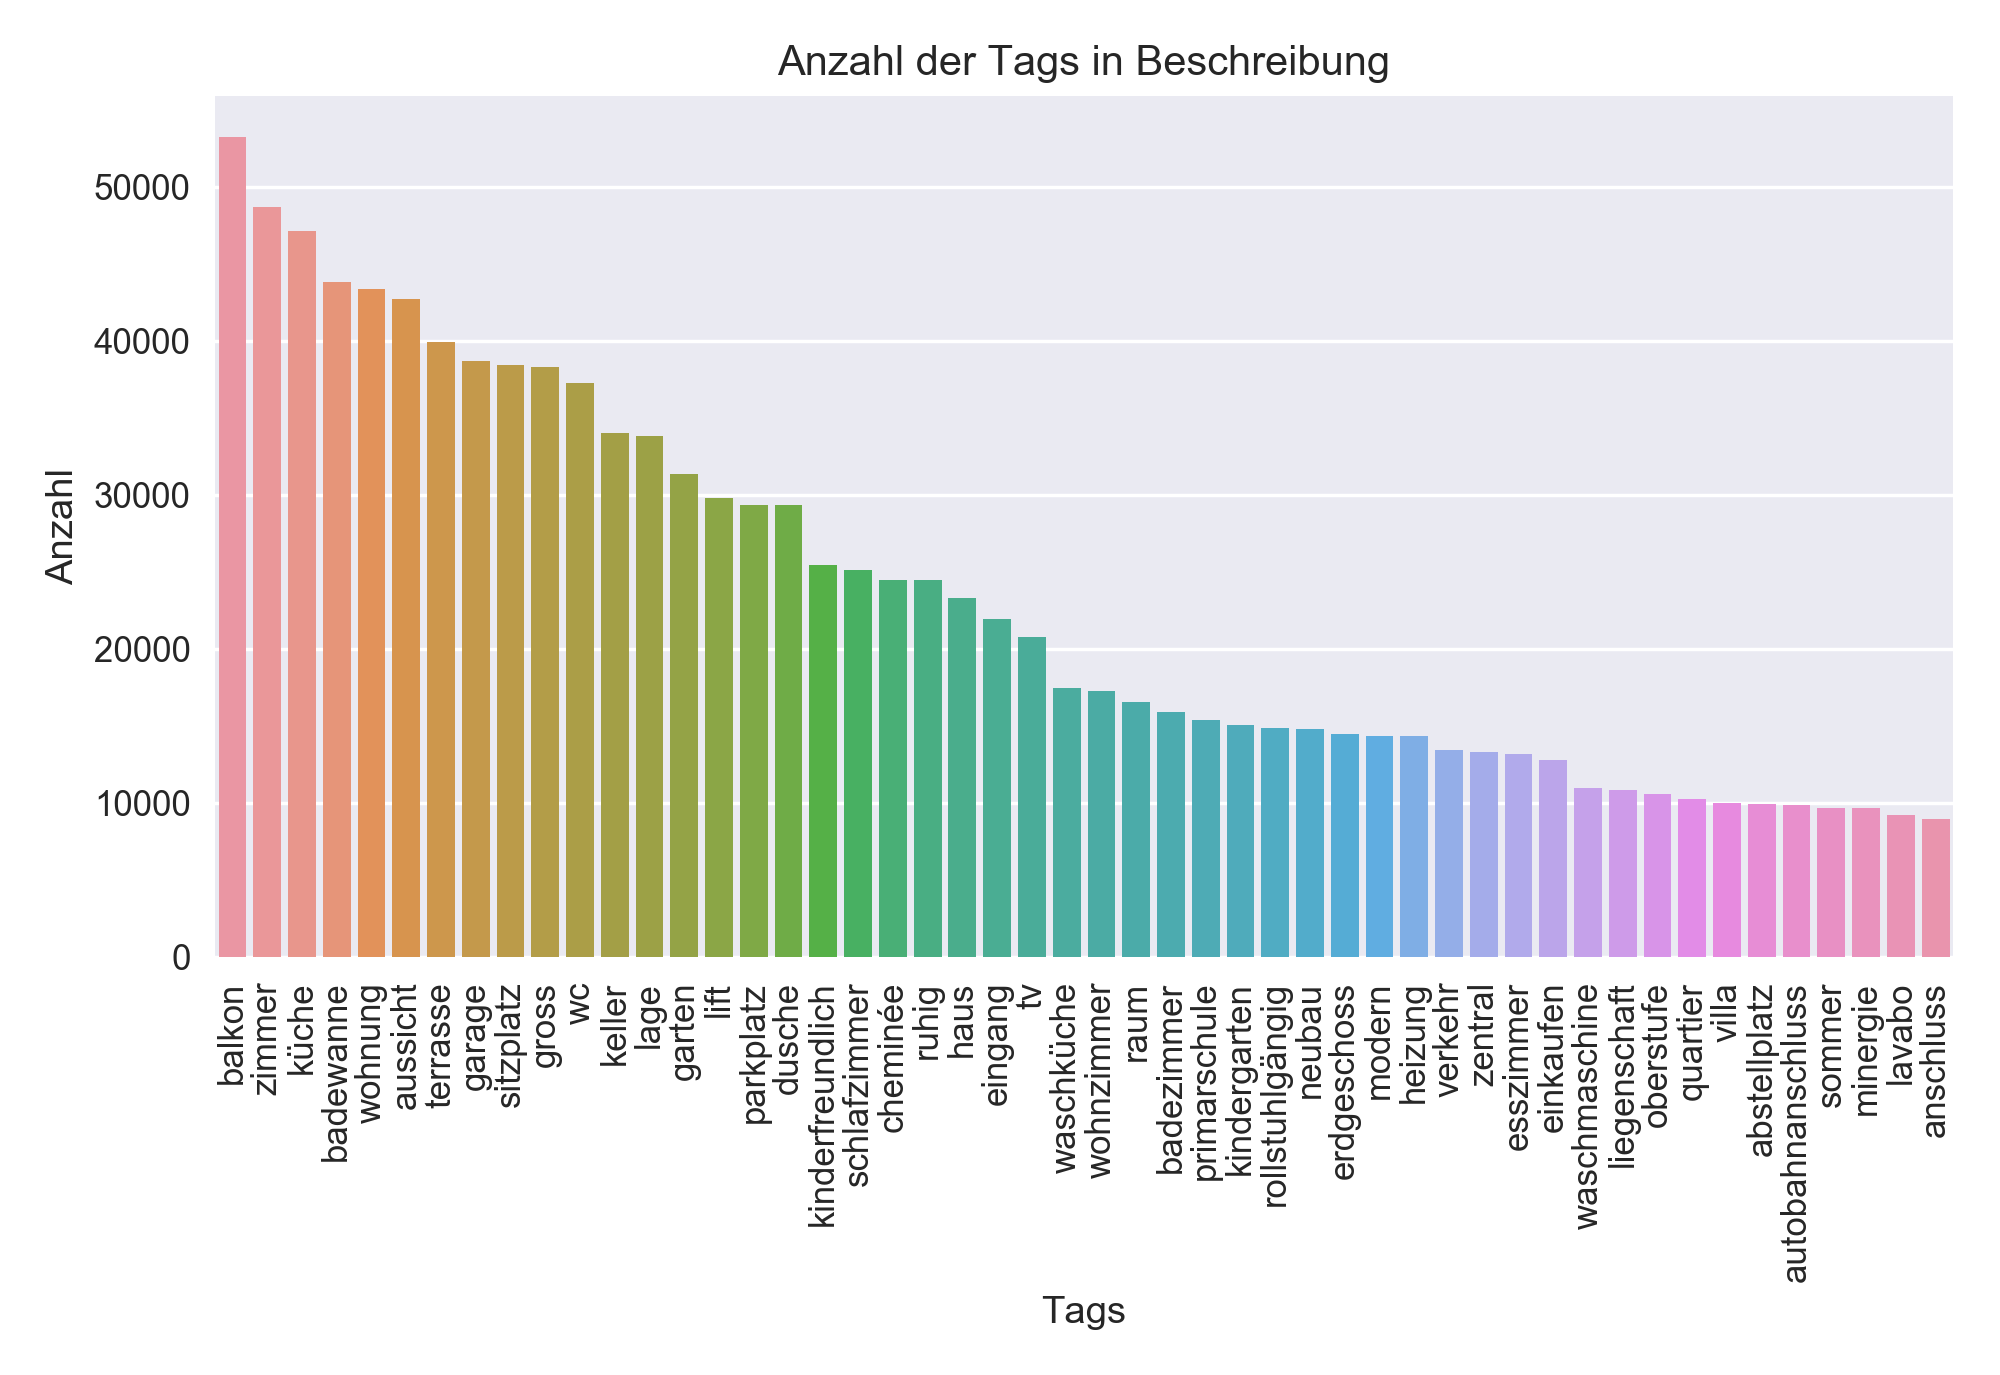
\includegraphics[width=\textwidth]{images/tags.png}
\caption[Die 50 häufigsten verwendeten Tags]{Die 50 häufigsten verwendeten Tags}%
\label{fig:tags}
\end{figure}

\subsection{Machine Learning}
Insgesamt haben wir neun verschiedene Machine Learning Algorithmen untersucht. Um eine vergleichnare Bewertung zu erhalten, bekamen alle Algorithmen die gleichen Datensätze zum Trainieren und zum Testen. So wurde verhindert, dass ein Algorithmus anhand eines vorteilhafteren Datensatzes eine bessere Performance erzielte. 

Als erstes bereiteten wir unsere gesammelten Daten für unsere Algorithmen auf. Dafür wurden die Features, wenn nötig, in nummerische Werte transformiert. Dies geschah im Feature Engineering. In den nächsten Absätzen werden die verschiedenen Algorithmen mit einem Basisdatensatz untersucht.

Als Basis für unseren Datensatz transformierten wir unsere kategorischen Features mit Hilfe einer One-Hot-Encoding in binäre Features um. So enstanden aus 35 Features über 2000 Features.\\
Wie im vorherigen Kapitel gezeigt, sind die Features Kubatur, Raumhöhe, effektive Fläche, Grundstücksfläche, Anzahl Stockwerke, Stockwerk und Renovationsjahr nur selten angegeben. Somit konnten sie nicht verwendet werden. Dafür konnten die Wohnfläche, die Anzahl Zimmer, das Baujahr, das Renovationsjahr, die Beschreibung und die Merkmale einer Immobile verwendet werden.\\
Als letzter Schritt wurden die Inserate gelöscht, die keinen Eintrag bei einem verwendeten Feature besassen oder doppelt vorkamen.

\subsubsection{Regressions Algorithmen}
Für die Auswertung der Algorithmen starteten wir mit den Regressions Algorithmen. Hierfür verwendeten wir eine  einfache lineare Regression, den Ridge- und den Lasso-Algorithmus. Die Ergebnisse werden in Tabelle \ref{tab:regression} aufgezeigt.

\begin{table*}[h]
\centering
\ra{1.3}
\resizebox{\textwidth}{!}{
\begin{tabular}{@{}lrrrrr@{}}
\toprule
ML Algorithmus & $R^2$ & MAPE & MdAPE & 10\% Abweichung & Maximaler Fehler\\
\midrule
Lineare Regression & -4.26E+25 & 2.93E+13 & 21.79 & 25.03 & 5.81E+20\\
Ridge Regression & 0.33 & 61.72 & 28.82 & 19.00 & 2.87E+07\\
Lasso Regression & 0.58 & 70.04 & 19.46 & 27.82 & 2.71E+07\\
\bottomrule
\end{tabular}}
\caption{Ergebnisse der Regression Algorithmen}
\label{tab:regression}
\end{table*}

Wir sehen, dass die Algorithmen eher schlecht abschnitten. Zum einen liegt das daran, dass noch kein richtiges Feature Engineering durchgeführt wurde. Zum anderen haben wir in unserem Modell sehr viele kategorische Features. Die lineare Regression erwartet eine Normalverteilung der Features, was bei kategorischen Features nicht der Fall ist.\\
Es ist ersichtlich, dass die Algorithmen mit einem Regularisierungsparameter eine deutlich bessere Performance erzielten, als die einfache lineare Regression. Somit ist ein Regularisierungsparameter bei diesem Datenset nützlich.\\
Auffallend war, dass der Lasso Algorithmus eine deutliche bessere Performance als der Ridge Algorithmus vorwies. Denn der Lasso kann unnötige Features eliminieren und somit die Komplexität reduzieren, während der Ridge immer alle Features verwenden muss. Abbildung \ref{fig:lasso} zeigt den Tukey-Anscombe Plot \ref{fig:lasso_tukey-anscombe} und die Verteilung der Residuen \ref{fig:lasso_histo}. Darauf ist ersichtlich, dass es extreme Ausreisser gibt und somit die MAPE verzerren.

\begin{figure}[h]
\begin{subfigure}{.5\textwidth}
  \centering
  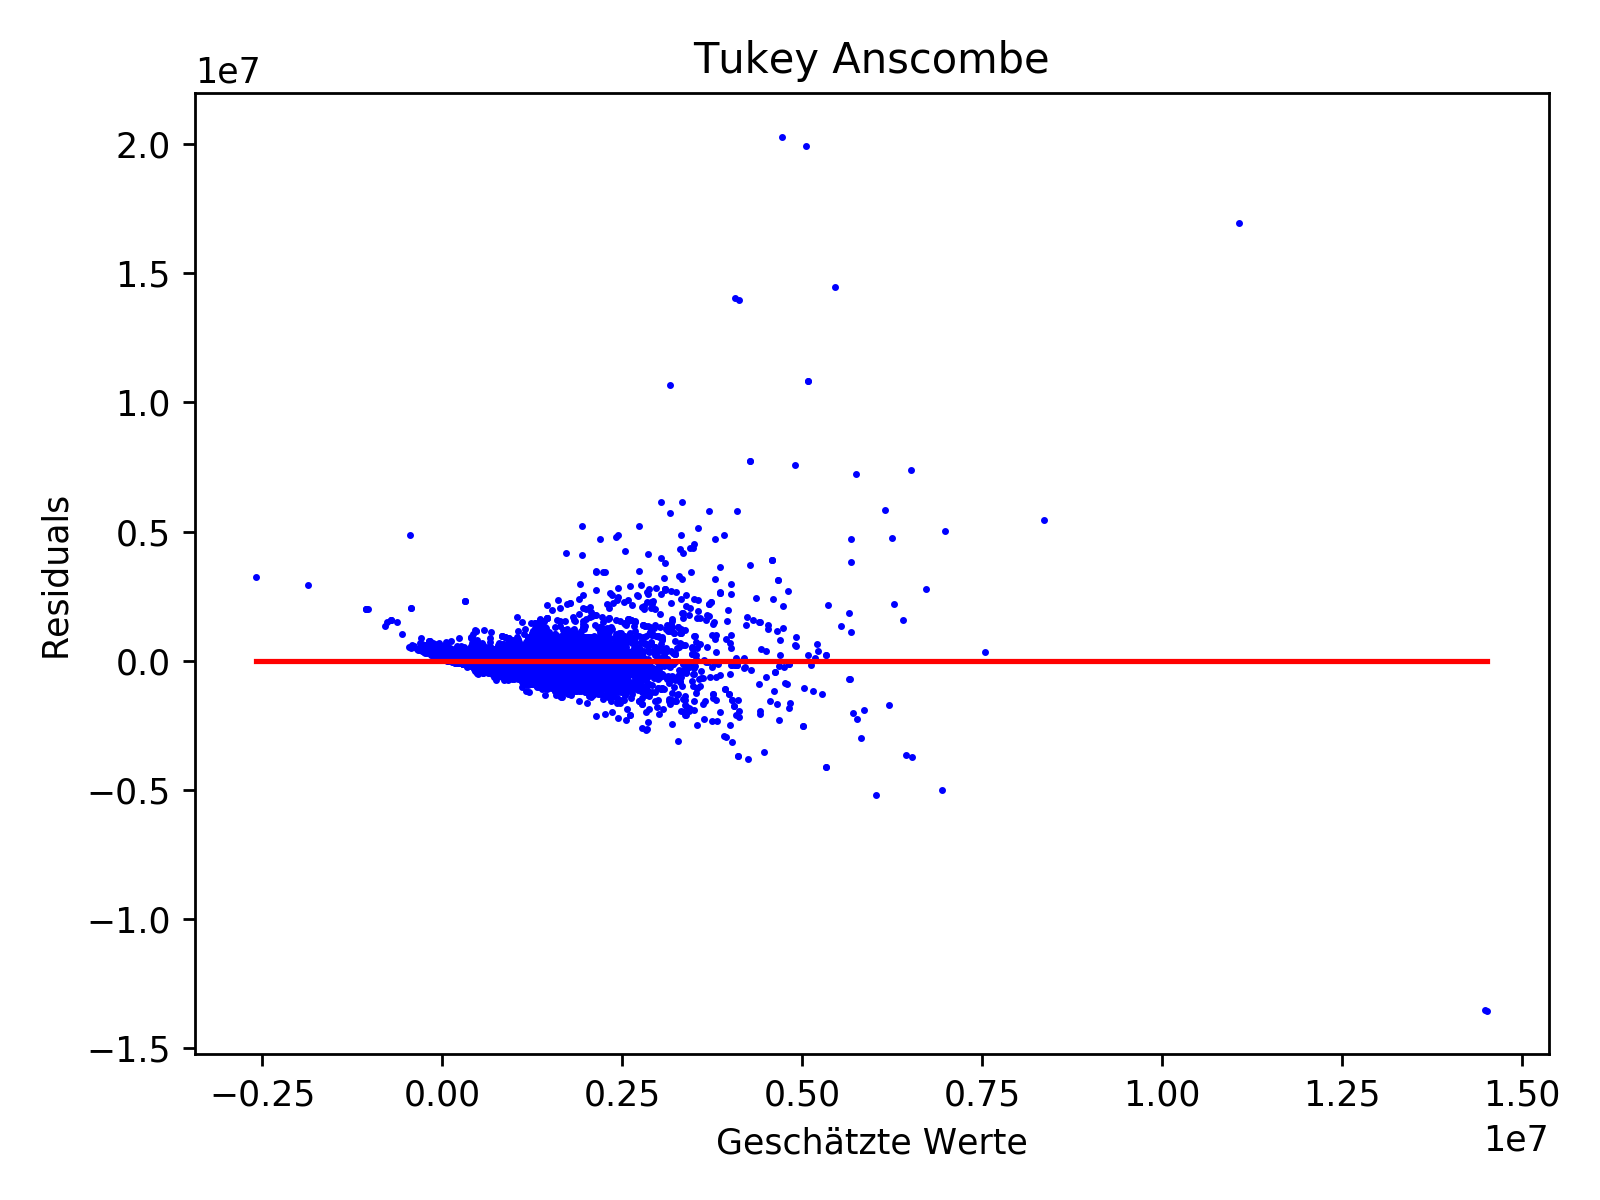
\includegraphics[width=\linewidth]{images/lasso_tukey.png}
  \caption[Tukey-Anscombe]{Tukey-Anscombe}
  \label{fig:lasso_tukey-anscombe}
\end{subfigure}
\begin{subfigure}{.5\textwidth}
  \centering
  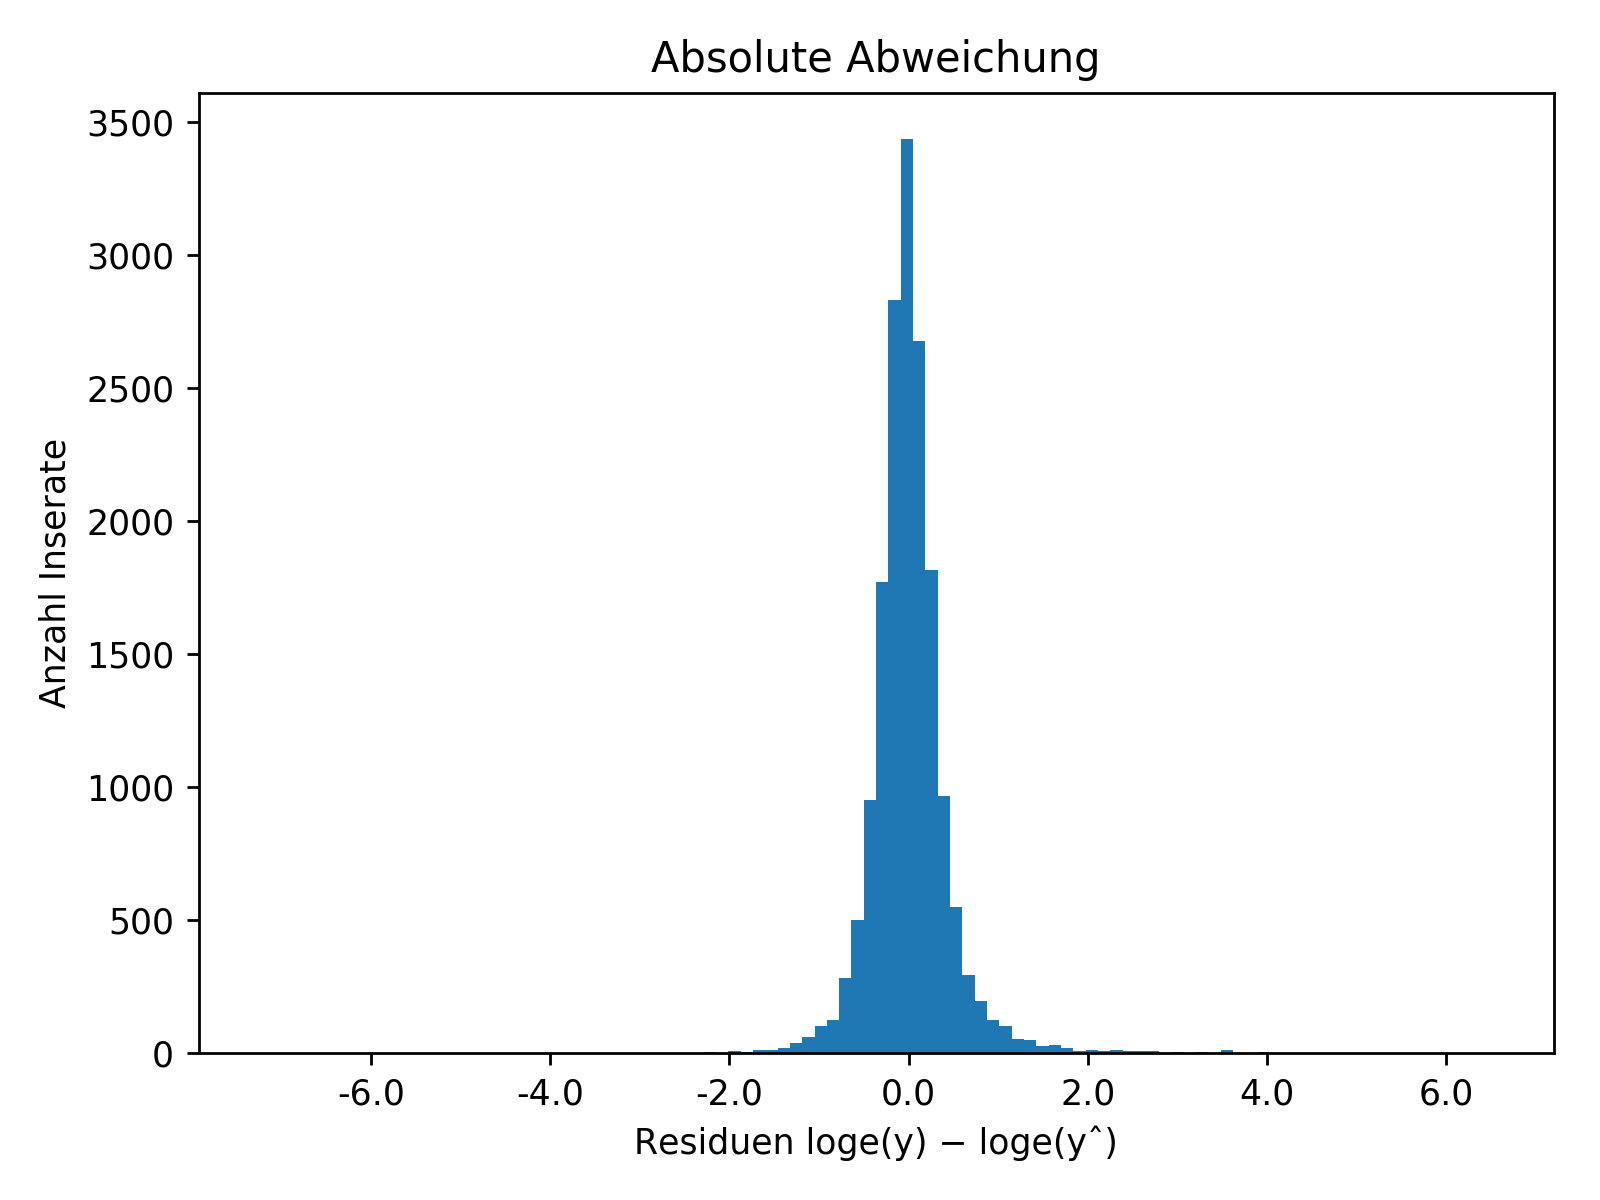
\includegraphics[width=\linewidth]{images/lasso_residuen.png}
  \caption[Histogramm]{Histogramm} % spaces needed for correct positioning
  \label{fig:lasso_histo}
\end{subfigure}
\caption[Auswertung der Residuen für Lasso]{Auswertung der Residuen für Lasso}
\label{fig:lasso}
\end{figure}

\subsubsection{$K$-Nearest Neighbour}
\label{chapter:KNN}
Beim nächsten Algorithmus handelte es sich um den $K$-Nearest Neighbour. Dieser Algorithmus, versucht anhand ähnlicher Inserate den Preis zu schätzen. Der Vorteil gegenüber den Regressions Algorithmen ist, dass es dem Algorithmus egal ist, in welchem Format die Features vorliegen. Zudem haben viele Features keinen negativen Einfluss auf den Algorithmus.
Tabelle \ref{tab:regression_knn} zeigt die erzielten Resultate an. Für die Berechnung wurden zwei Nachbarn zum Vergleich, eine Leaf size von 100 und für die Gewichtung die Euklid-Distanz verwendet.

\begin{table*}[ht]
\centering
\ra{1.3}
\resizebox{\textwidth}{!}{
\begin{tabular}{@{}lrrrrr@{}}
\toprule
ML Algorithmus & $R^2$ & MAPE & MdAPE & 10\% Abweichung & Maximaler Fehler\\
\midrule
$K$-Nearest Neighbour & 0.83 & 23.67 & 0 & 79.94 & 1.81E+07\\
\bottomrule
\end{tabular}}
\caption{Ergebnisse von $K$-Nearest Neighbour}
\label{tab:regression_knn}
\end{table*}

Die Performance wurde deutlich besser als bei den Regressions Algorithmen. 79,94\% der Immobilien konnten mit einer Abweichung von 10\% richtig geschätzt werden. Anhand diesen Ergebnissen konnte aufgezeigt werden, dass bei ähnlichen Immobilien auch ein ähnlicher Preis existiert.\\
Eine MdAPE von 0\% erklärten wir damit, dass es sehr ähnliche Häuser gibt, die den selben Preis besitzen. Wir gehen im Kapitel 5 nochmals genauer darauf ein. Die MAPE mit einem Wert von 23,67\% war zu hoch, um von einem guten Modell zu sprechen. Abbildung \ref{fig:kneighbour} zeigt die Statistik für die Residuen. Im Histogramm \ref{fig:kneighbour_histo} wird nochmals der MdAPE von 0\% deutlich. Auf dem Tukey-Anscombe Plot \ref{fig:kneighbour_tukey-anscombe} wichen die Residuen weniger stark vom beobachteten Preis ab als beim Lasso.

\begin{figure}[h]
\begin{subfigure}{.5\textwidth}
  \centering
  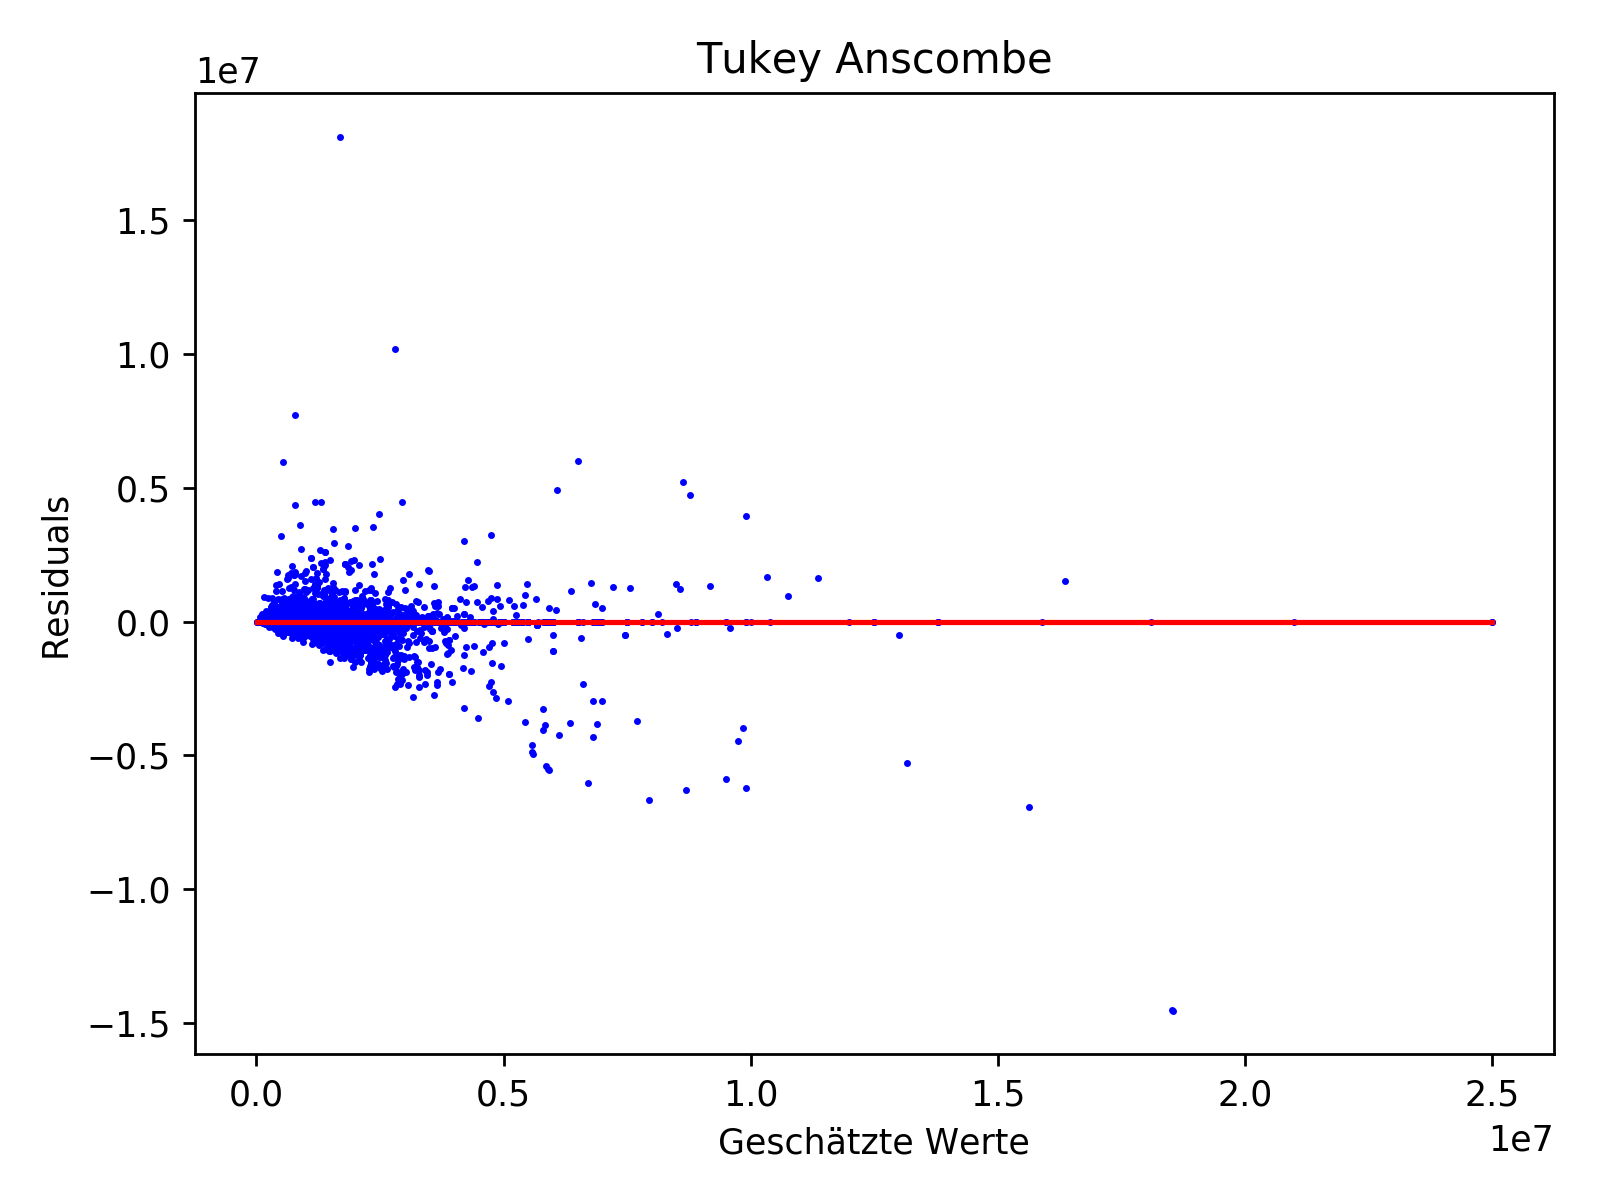
\includegraphics[width=\linewidth]{images/KNeighbour_tukey.png}
  \caption[Tukey-Anscombe]{Tukey-Anscombe}
  \label{fig:kneighbour_tukey-anscombe}
\end{subfigure}
\begin{subfigure}{.5\textwidth}
  \centering
  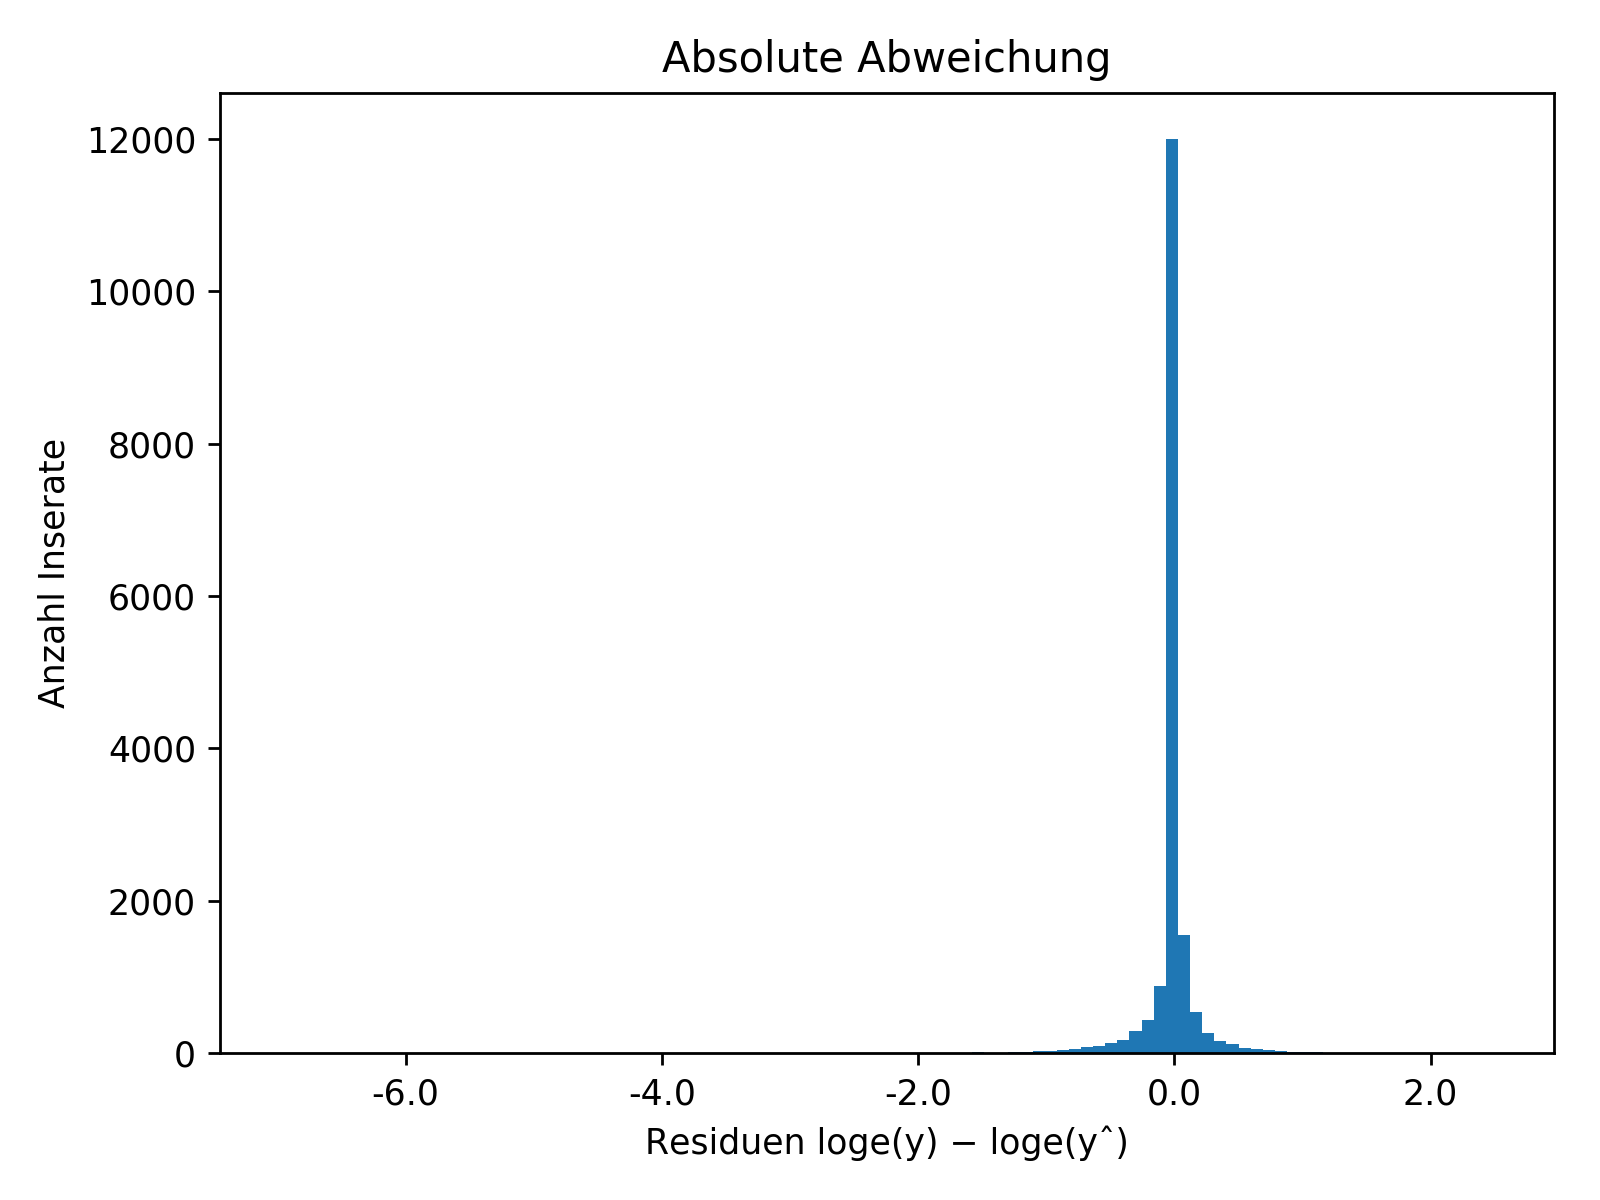
\includegraphics[width=\linewidth]{images/KNeighbour_residuen.png}
  \caption[Histogramm]{Histogramm}
  \label{fig:kneighbour_histo}
\end{subfigure}
\caption[Auswertung der Residuen für KNN]{Auswertung der Residuen für KNN}
\label{fig:kneighbour}
\end{figure}

\subsubsection{Baum Algorithmen}
Als nächstes untersuchten wir verschiedene Baum Algorithmen. Diese erfreuen sich aktuell einer grosser Beliebtheit bei diversen Machine Learning Wettbewerben\footnote{https://www.kaggle.com/c/house-prices-advanced-regression-techniques}.\\[2ex]
%
Wir haben vier verschiedene Algorithmen untersucht. Sie unterscheiden sich hauptsächlich in ihrer Strategie. Der Random Forest wendet eine Art Bagging an. Der XGBoost wie auch der AdaBoost verwenden eine Boostingstrategie und der Extra Trees verwendet weder Boosting noch Bagging.

Eine Auswertung mittels GridSearchCV hatte für die Algorithmen folgende Parameter vorgeschlagen.
Für Random Forest verwendeten wir 700 Schätzungsmodelle, ansonsten die Default Parameter von Scikit Learn. Dasselbe galt auch für den Extra Trees Algorithmus.\\
Für AdaBoost haben wir als Basis Schätzungsmodell den DecisionTreeRegressor mit 18 Schätzungsmodelle benutzt.\\
Der XGBoost besass eine maximale Tiefe von 100 mit einer Lernrate von 0.1 und 350 Schätzungsmodelle.

\begin{table*}[ht]
\centering
\ra{1.3}
\resizebox{\textwidth}{!}{
\begin{tabular}{@{}lrrrrr@{}}
\toprule
ML Algorithmus & $R^2$ & MAPE & MdAPE & 10\% Abweichung & Maximaler Fehler\\
\midrule
Random Forest & 0.907 & 23.31 & 2.43 & 77.52 & 1.26E+07\\
Extra Trees & 0.91 & 23.88 & 0.86 & 81.74 & 1.04E+07\\
XGBoost & 0.898 & 18.71 & 0.81 & 82.01 & 1.46E+07\\
AdaBoost & 0.907 & 18.14 & 0.00 & 83.69 & 1.63E+07\\
\bottomrule
\end{tabular}}
\caption{Ergebnisse der Baum Algorithmen}
\label{tab:first_round}
\end{table*}

In Tabelle \ref{tab:first_round} ist erkennbar, dass die Baum Algorithmen, bis auf den Random Forest, eine noch bessere Performance hatten, als der $K$-Nearest Neighbour. Die vielen kategorischen Features halfen den Baumalgorithmen eine gute Performance zu erzielen. Wie beim $K$-Nearest Neighbour war die MAPE zu hoch, um von einem guten Modell zu sprechen.\\
Abbildung \ref{fig:adaboost_1} zeigt die Resultate für AdaBoost, da dieser die besten Resultate erzielte. Gros­so mo­do waren die Resultate ähnlich dem KNN. Wie im Tukey-Anscombe Plot \ref{fig:ada_tukey-anscombe_1} dargestellt, existierten weniger starke Ausreisser und die Residuen waren näher am Beobachtungswert. Das Histogramm \ref{fig:ada_histo_1} unterschied sich nicht gross vom KNN.

\begin{figure}[h]
\begin{subfigure}{.5\textwidth}
  \centering
  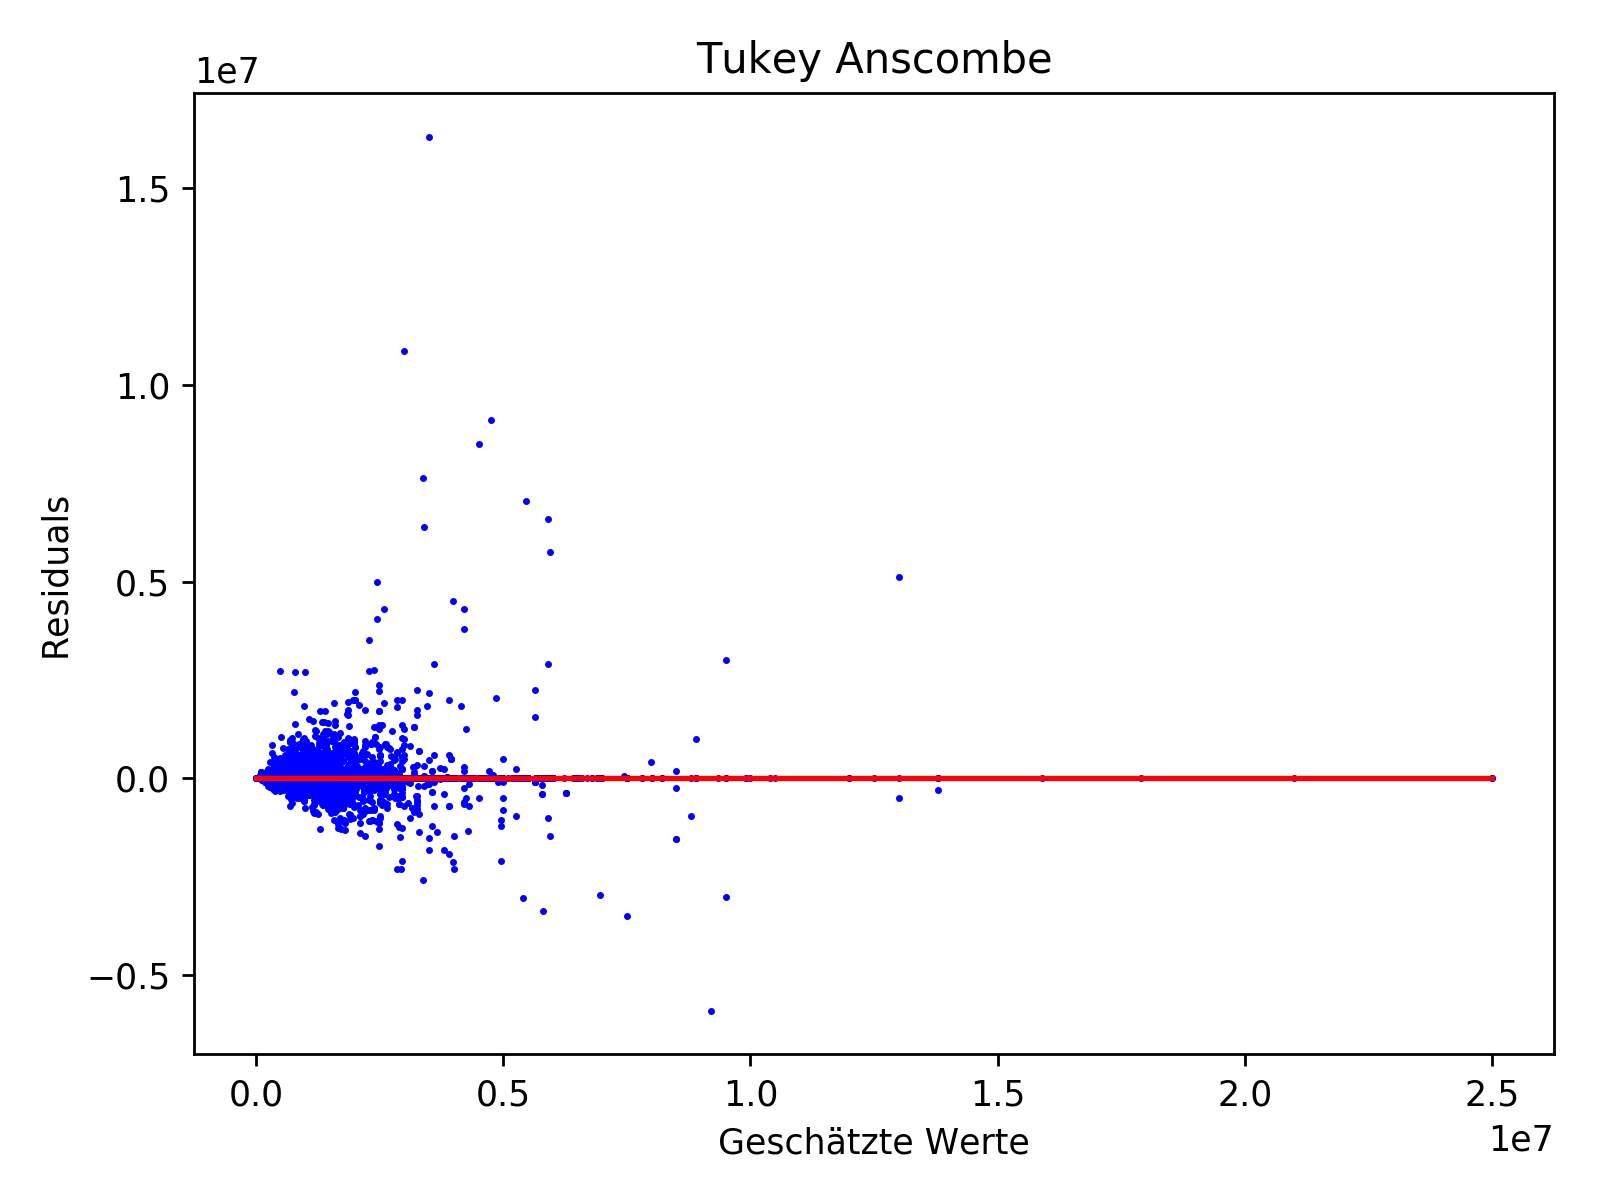
\includegraphics[width=\linewidth]{images/adaboost_tukey_anscombe_1.png}
  \caption[Tukey-Anscombe]{Tukey-Anscombe}
  \label{fig:ada_tukey-anscombe_1}
\end{subfigure}
\begin{subfigure}{.5\textwidth}
  \centering
  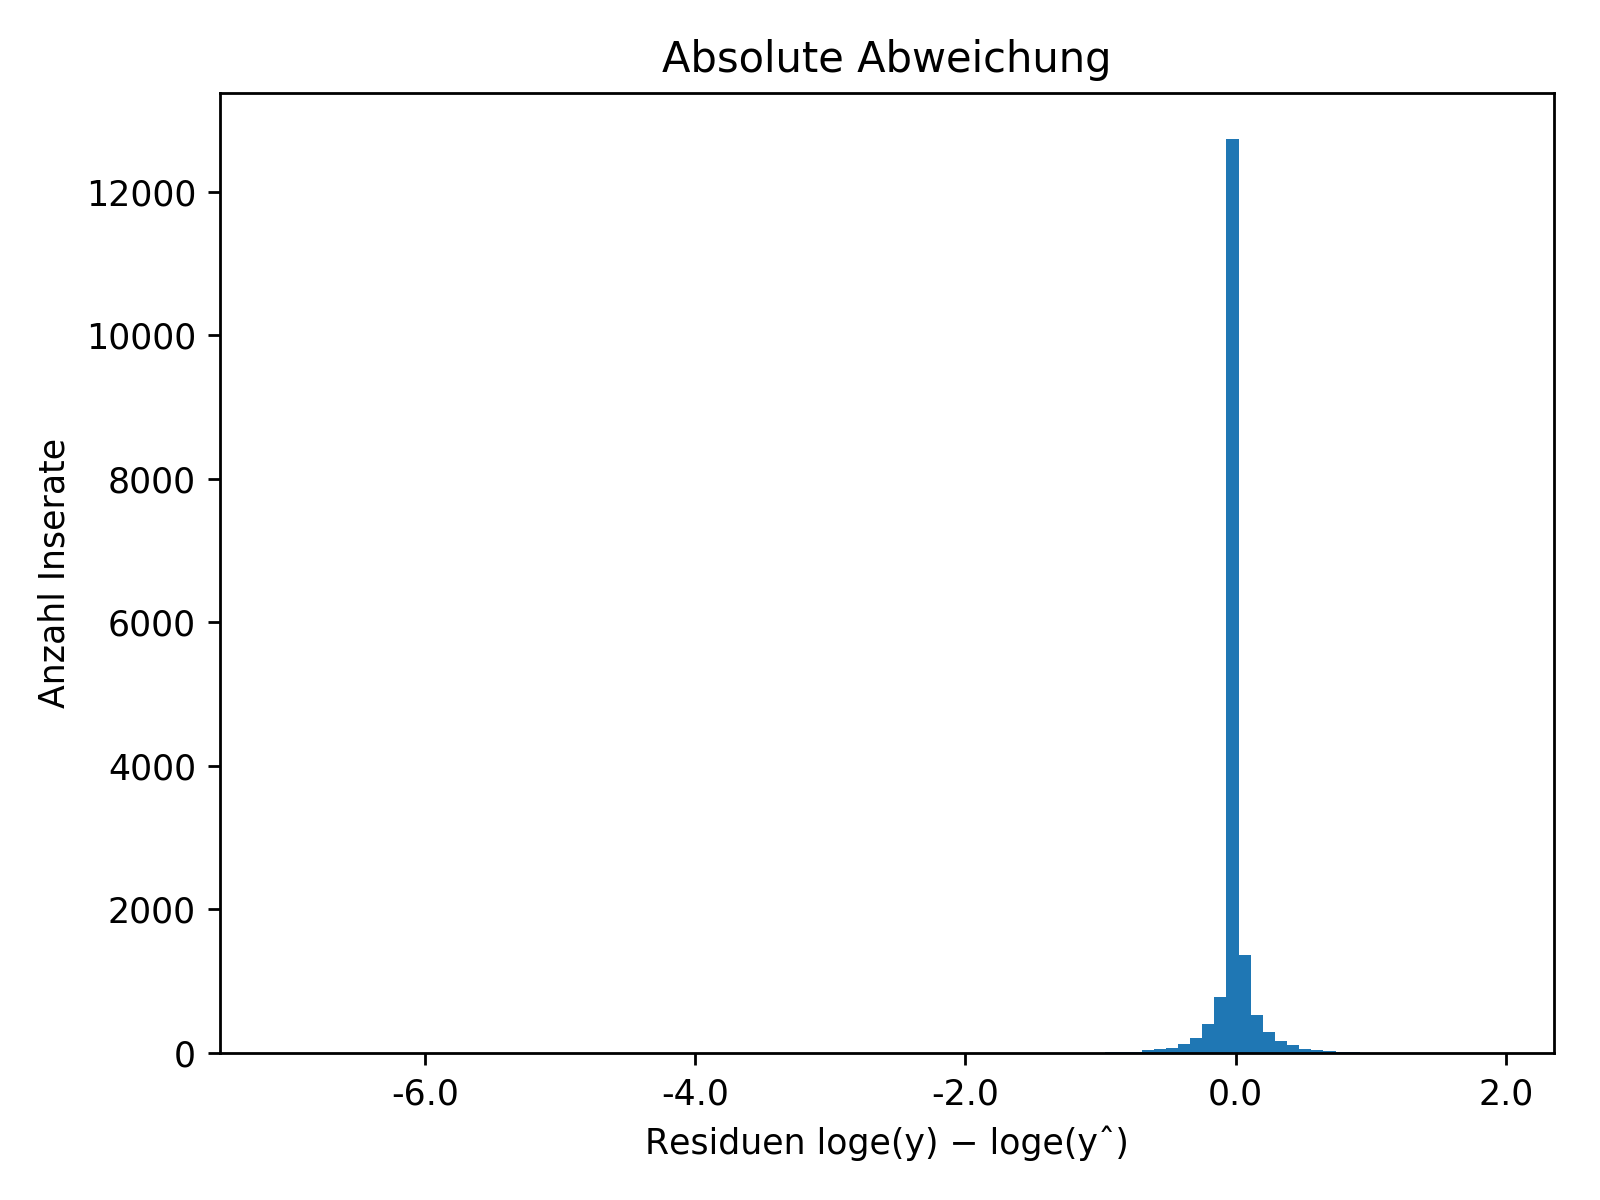
\includegraphics[width=\linewidth]{images/adaboost_verteilung_residuals_log_1.png}
  \caption[Histogramm]{Histogramm}
  \label{fig:ada_histo_1}
\end{subfigure}
\caption[Auswertung der Residuen für AdaBoost]{Auswertung der Residuen für AdaBoost}
\label{fig:adaboost_1}
\end{figure}

Für das weitere Vorgehen wurden nur noch der Extra Trees, XGBoost und der AdaBoost verwendet, da diese die besten Werte erreichten.
% - - - - - - - - - - - - - -
% Feature engineering
% - - - - - - - - - - - - - -
\subsubsection{Feature Engineering}
Um eine bessere Performance zu erhalten, wurde anhand von Feature Engineering versucht weitere Features zu generieren. Aus den beiden Features Wohnfläche und Anzahl Zimmer, berechneten wir die durchschnittliche Zimmergrösse. Wir nahemn diese beiden Features, da diese eine hohe Korrelation mit dem Preis besassen. Tabelle \ref{tab:second_round} zeigt die Ergebnisse auf.

\begin{table*}[ht]
\centering
\ra{1.3}
\resizebox{\textwidth}{!}{
\begin{tabular}{@{}lrrrrr@{}}
\toprule
ML Algorithmus & $R^2$ & MAPE & MdAPE & 10\% Abweichung & Maximaler Fehler\\
\midrule
Extra Trees & 0.903 & 27.14 & 0.82 & 81.426 & 1.76E+07\\
XGBoost & 0.888 & 25.27 & 0.752 & 81.94 & 2.30E+07\\
AdaBoost & 0.885 & 23.28 & 0 & 83.97 & 2.33E+07\\
\bottomrule
\end{tabular}}
\caption{Ergebnisse mit durchschnittlicher Zimmergrösse}
\label{tab:second_round}
\end{table*}

Erstaunlicherweise konnte sich kein Algorithmus verbessern. Im Gegenteil, die Schätzungen wurden schlechter, obwohl die durchschnittliche Zimmergrösse als drittwichtigstes Feature gewichtet wurde. Die maximale Abweichung von 10\% ist jedoch gleich gut geblieben. Aus diesem Grund verwendeten wir dieses Feature weiterhin für die Erstellung unsers Modells. Die höhere MAPE erklärten wir uns durch den höheren maximalen Fehler.\\
Interessanterweise besassen Wohnfläche, Anzahl Zimmer und durchschnittliche Zimmergrösse eine hohe Gewichtung, obwohl sie untereinander eine starke Korrelation aufwiesen. Normalerweise erhält nur ein Feature von mehreren stark korrelierende Features eine hohe Gewichtung.\\[2ex]
%
\textbf{Renovationsjahr}\\
Als nächstes ergänzten wir die bestehenden Features durch ein binäres Feature, das auf 1 steht, falls eine Renovation durchgeführt wurde und andernfalls auf 0 steht.\\
Zusätzlich berechneten wir die Anzahl Jahre seit der letzten Renovation. Fehlte das Renovationsjahr, wurde stattdessen das Baujahr verwendet. Durch die Transformation fiel das Renovationsjahr weg. Die Ergebnisse sind in Tabelle \ref{tab:third_round} dargestellt.

\begin{table*}[ht]
\centering
\ra{1.3}
\resizebox{\textwidth}{!}{
\begin{tabular}{@{}lrrrrr@{}}
\toprule
ML Algorithmus & $R^2$ & MAPE & MdAPE & 10\% Abweichung & Maximaler Fehler\\
\midrule
Extra Trees & 0.915152 & 20.048 & 0.87 & 81.804 & 8.87E+06\\
XGBoost & 0.910506 & 20.191 & 0.802 & 82.113 & 9.19E+06\\
AdaBoost & 0.920327 & 18.484 & 0 & 83.528 & 9.75E+06\\
\bottomrule
\end{tabular}}
\caption{Ergebnisse mit Einbezug der Renovation}
\label{tab:third_round}
\end{table*}

Obwohl das Renovationsjahr keine starke Korrelation mit dem Kaufpreis besass, konnten diese beiden Features die Performance unserer Modelle verbessern. Zusätzlich konnte der maximale Fehler um einiges verringert werden, was einen positiven Einfluss auf die MAPE hatte. Die maximale Abweichung von 10\% ist jedoch gleich geblieben.

\textbf{Lärmbelastung}\\
Für die Berechnung der Lärmbelastung nahmen wir den Durchschnitt von 255 Pixel, was etwa einem Radius von 10m entspricht. Fehlte die exakte Wohnadresse, verwendeten wir die Koordinaten der Gemeinde.\\
Abbildung \ref{fig:noise} zeigt einen Ausschnitt der Lärmkarte für eine Berechnung der Lärmbelastung. Tabelle \ref{tab:fourth_round} zeigt die Ergebnisse der Modelle, mit dem neuen Feature Lärmbelastung.

\begin{figure}[ht]
\centering
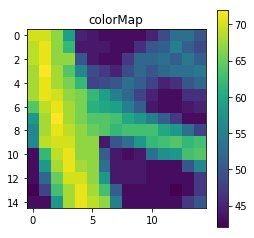
\includegraphics[width=0.5\textwidth]{images/noise.jpeg}
\caption[Ausschnitt der Lärmbelastung am Brausebad (Basel)]{Ausschnitt der Lärmbelastung am Brausebad (Basel)}
\label{fig:noise}
\end{figure}

\begin{table*}[ht]
\centering
\ra{1.3}
\resizebox{\textwidth}{!}{
\begin{tabular}{@{}lrrrrr@{}}
\toprule
ML Algorithmus & $R^2$ & MAPE & MdAPE & 10\% Abweichung & Maximaler Fehler\\
\midrule
Extra Trees & 0.838332 & 9.912 & 0.85 & 82.002 & 2.79E+07\\
XGBoost & 0.814466 & 9.952 & 0.74 & 82.212 & 2.81E+07\\
AdaBoost & 0.823295 & 9.954 & 0 & 83.593 & 2.75E+07\\
\bottomrule
\end{tabular}}
\caption{Ergebnisse mit Einbezug der Lärmbelastung}
\label{tab:fourth_round}
\end{table*}

In diesem Durchlauf hatte sich die MAPE beträchtlich verbessert, obwohl der maximale Fehler sehr hoch ist. Die MdAPE sowie die maximale Abweichung von 10\% wurden leicht besser.

\newpage
\textbf{Outlier Detection}\\
Auffallend war, dass bei allen Modellen der hohe maximale Fehler zwischen 10 und 25 Millionen lag. Um diesen Fehler zu verkleinern führten wir vor dem Lernen eine Outlier Detection durch. Somit wurden Immobilien mit abnormalen Werten aus dem Datensatz entfernt.\\
Für die Outlier Detection wendeten wir den Isolation Forest auf unsere numerischen Features an. So konnten wir fehlerhafte Inserate erkennen und entfernen.\\[2ex]
%
Beim Isolation Forest definiert ein Prozentsatz die Anzahl an markierten Ausreisser.
Um einen geeigneten Prozentsatz zu bestimmen, verglichen wir die Entwicklung der Standardabweichung bei Erhöhung des Prozentsatzes.\\
War die Differenz der Standardabweichung mit der Vorherigen nicht um mehr als 2.5\% gesunken, hatten wir unseren optimalen Prozentsatz gefunden.\\
Die 2.5\% ergaben bei uns die richtige Mischung aus genügend erkannten Ausreissern, ohne, dass zu viele Inserate entfernt wurden.
Abbildung \ref{fig:outlier} zeigt die Reduktion der Standardabweichung \ref{fig:isolation_std} und die gefundenen Outlier \ref{fig:isolation_forest} bei der Wohnfläche. Tabelle \ref{tab:iso_forest} zeigt die gefunden Ausreisser im Datensatz. Insgesamt wurden 12'362 Inserate als Ausreisser markiert und entfernt. 
Es ist unschwer zu erkennen, dass gewisse Inserate nicht nur bei einem Feature als Ausreisser markiert wurden, sondern gleich bei mehreren.

\begin{figure}[ht]
\begin{subfigure}{.5\textwidth}
  \centering
  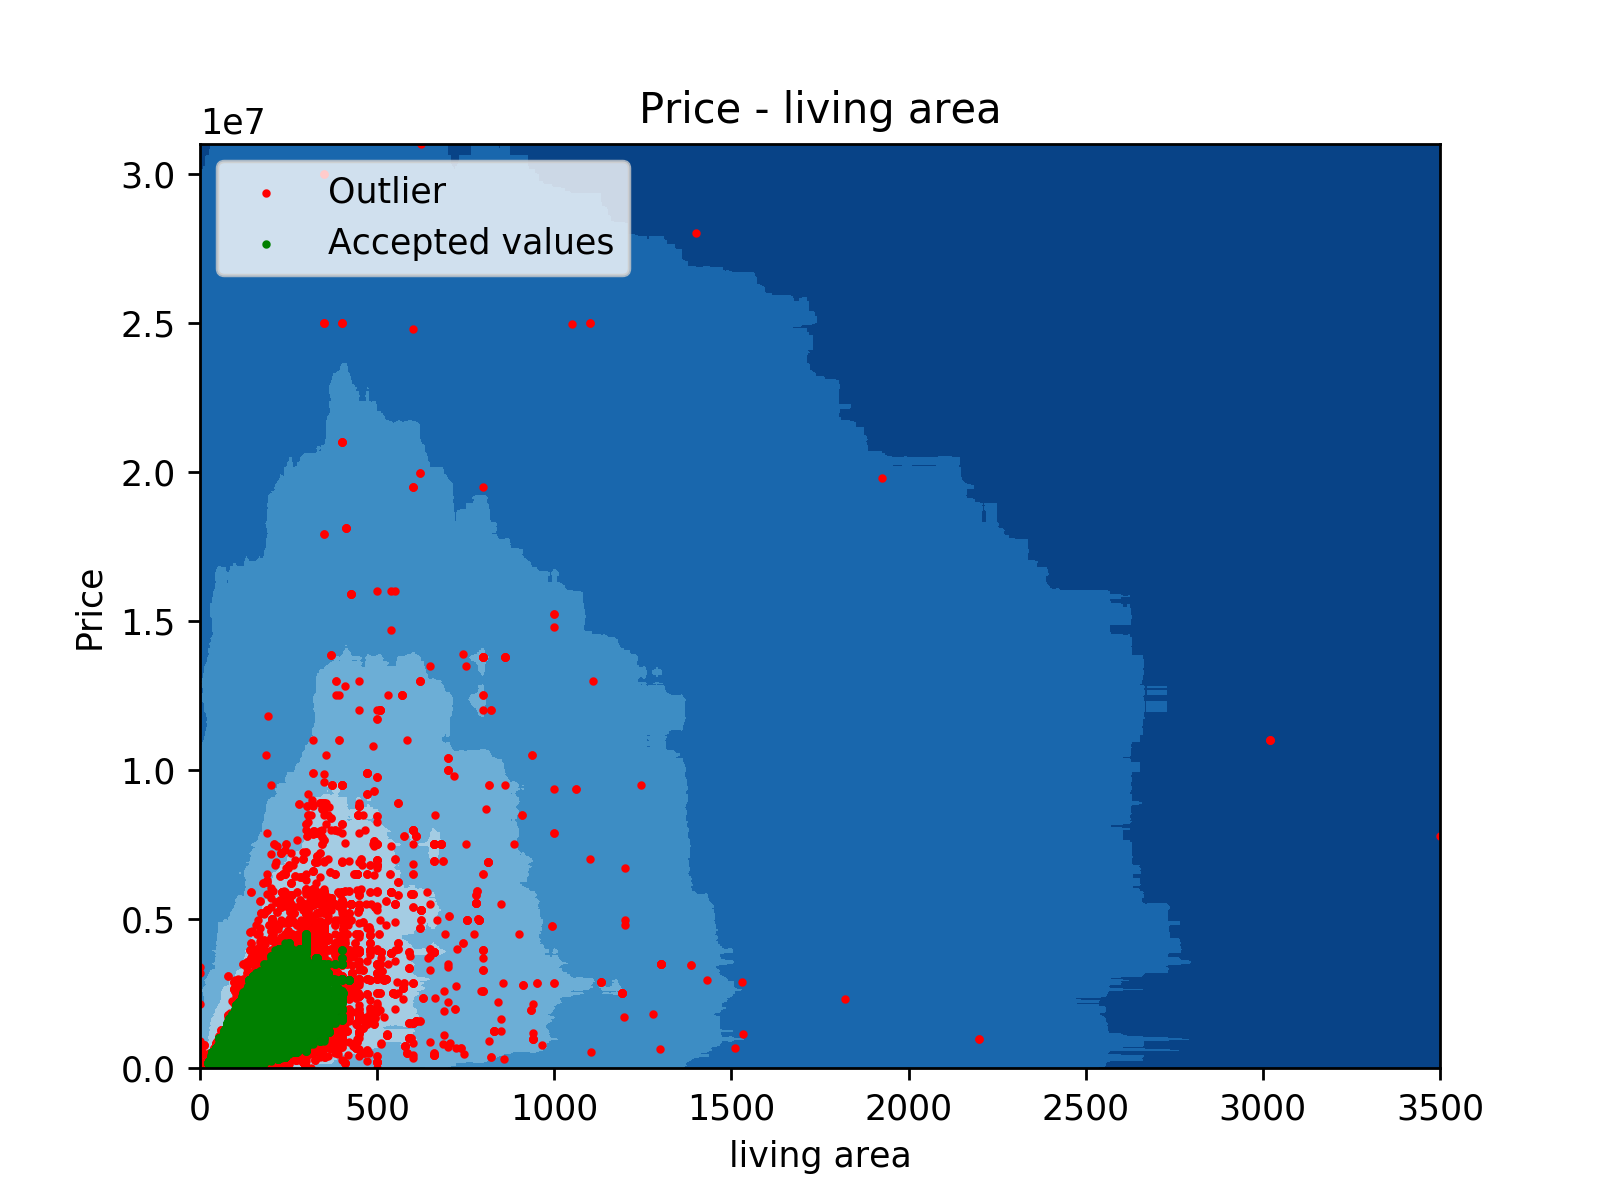
\includegraphics[width=\linewidth]{images/living_area_IsolationForest.png}
  \caption[Isolation Forest angewendet auf Wohnfläche]{Isolation Forest angewendet auf Wohnfläche}
  \label{fig:isolation_forest}
\end{subfigure}
\begin{subfigure}{.5\textwidth}
  \centering
  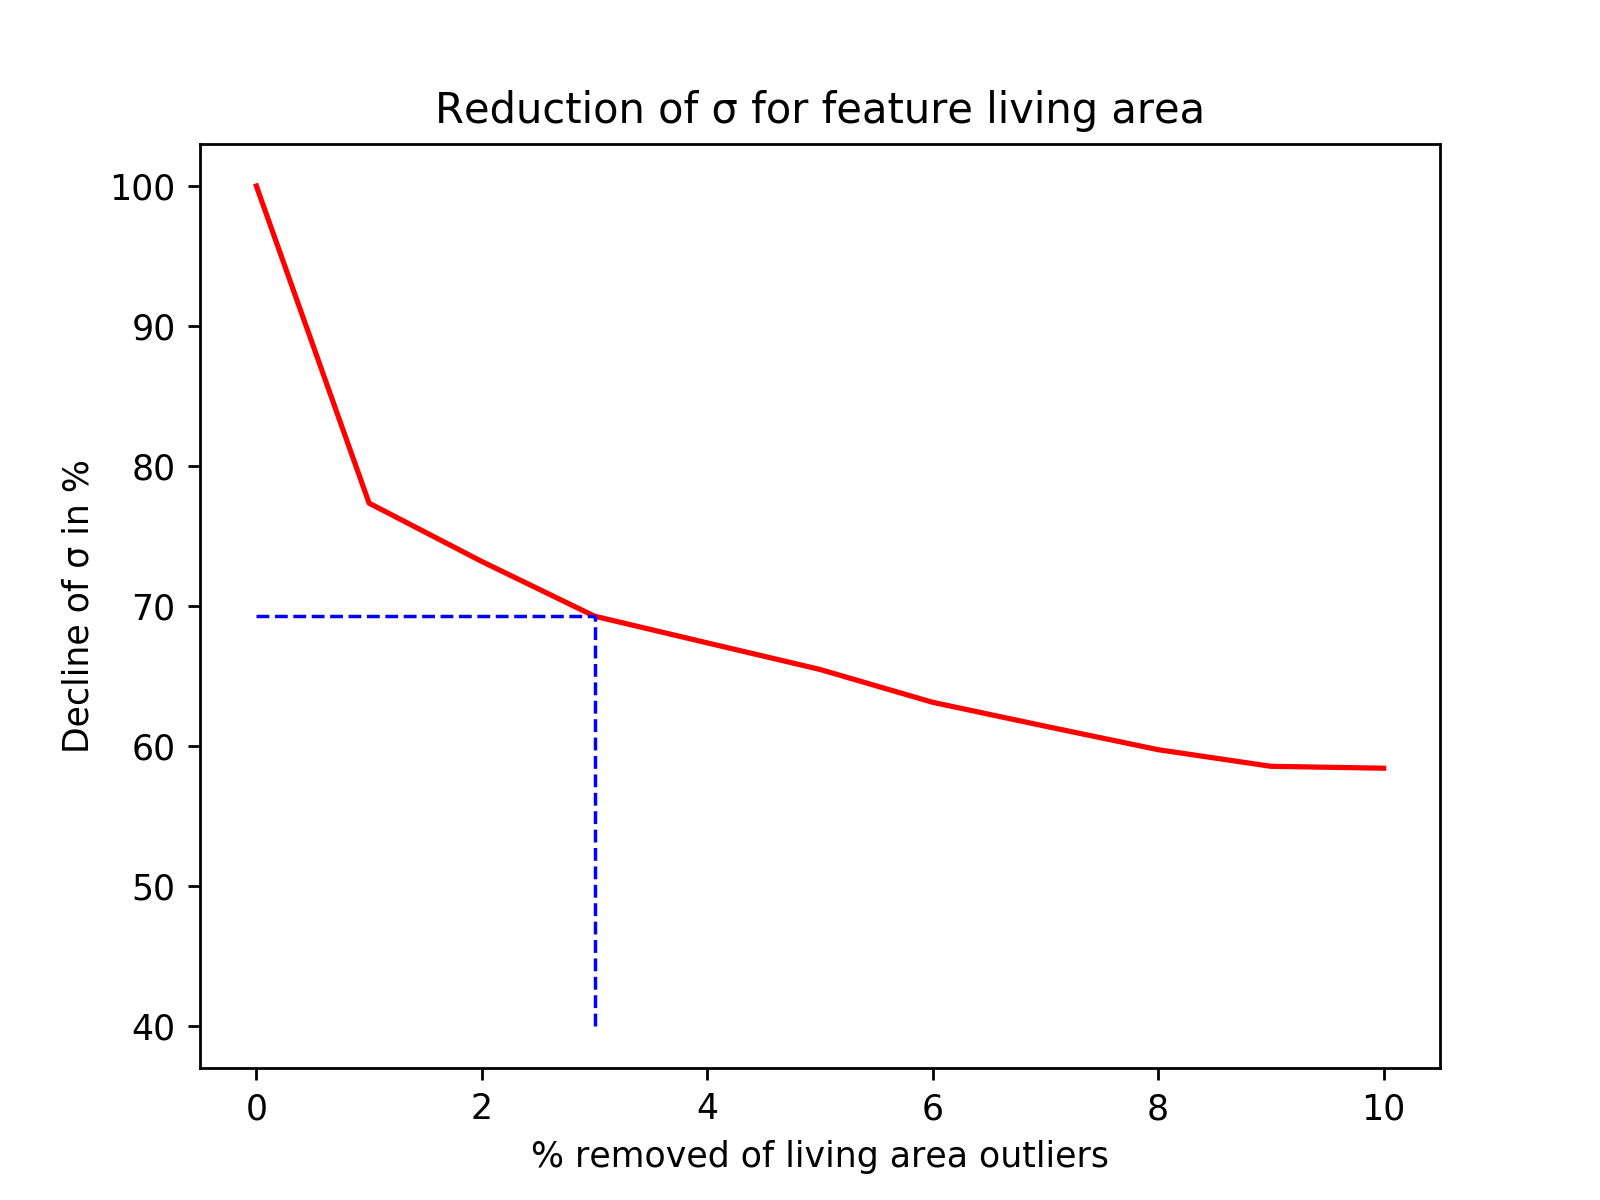
\includegraphics[width=\linewidth]{images/living_area_std.png}
  \caption[Entwicklung der Standardabweichung]{Entwicklung der Standardabweichung\\ \ } % spaces needed for correct positioning
  \label{fig:isolation_std}
\end{subfigure}
\caption[Outlier Detection: Wohnfläche]{Outlier Detection: Wohnfläche}
\label{fig:outlier}
\end{figure}

\begin{table*}[ht]
\centering
\ra{1.3}
\begin{tabular}{@{}lrr@{}}
\toprule
Feature & Entfernt in \% & \# entfernte Inserate\\
\midrule
Baujahr & 5 & 4293\\
Anzahl Zimmer & 3 & 2579\\
Wohnfläche & 3 & 2577\\
Letzte Konstruktion & 5 & 4294\\
Lärmbelastung & 7 & 7726\\
\bottomrule
\end{tabular}
\caption{Übersicht der entfernten Inserate mit dem Isolation Forest}
\label{tab:iso_forest}
\end{table*}
%
\begin{table*}[ht]
\centering
\ra{1.3}
\resizebox{\textwidth}{!}{
\begin{tabular}{@{}lrrrrr@{}}
\toprule
ML Algorithmus & $R^2$ & MAPE & MdAPE & 10\% Abweichung & Maximaler Fehler\\
\midrule
Extra Trees & 0.947074 & 5.216 & 0.702 & 84.269 & 1.89E+06\\
XGBoost & 0.941227 & 5.392 & 0.604 & 84.208 & 1.95E+06\\
AdaBoost &0.940529 & 4.692 & 0 & 85.609 & 1.95E+06\\
\bottomrule
\end{tabular}}
\caption{Ergebnisse mit Einbezug einer Outlier Detection}
\label{tab:fifth_round}
\end{table*}

Wird die Einführung der Outlier Detection auf die Performance der Algorithmen in Tabelle \ref{tab:fifth_round} betrachtet, ist erkennbar, dass bei allen Performancekriterien eine Verbesserung erzielt werden konnte. Der maximale Fehler wurde auf 2~Mio.~CHF verkleinert, da Extremwerte nicht mehr vorhanden waren. Deshalb ist eine Outlier Detection für ein Machine Learning Algorithmus essentiell. Dies ist auch in Abbildung \ref{fig:adaboost_6} beim Tukey-Anscombe Plot \ref{fig:ada_tukey-anscombe_6} wie auch beim Histogramm der Residuen \ref{fig:ada_histo_6} ersichtlich.

Die Tabelle \ref{tab:price_outlier} zeigt die neuen statistischen Werte für den Kaufpreis einer Immobilie. Im Vergleich zu Tabelle \ref{tab:price} ist ersichtlich, dass die Standardabweichung beträchtlich vermindert wurde. Ebenso ergeben der minimale wie auch der maximale Preis mehr Sinn. Der Durchschnitt und der Median besitzen ähnliche Werte wie vor der Outlier Detection.

\begin{figure}[h]
\begin{subfigure}{.5\textwidth}
  \centering
  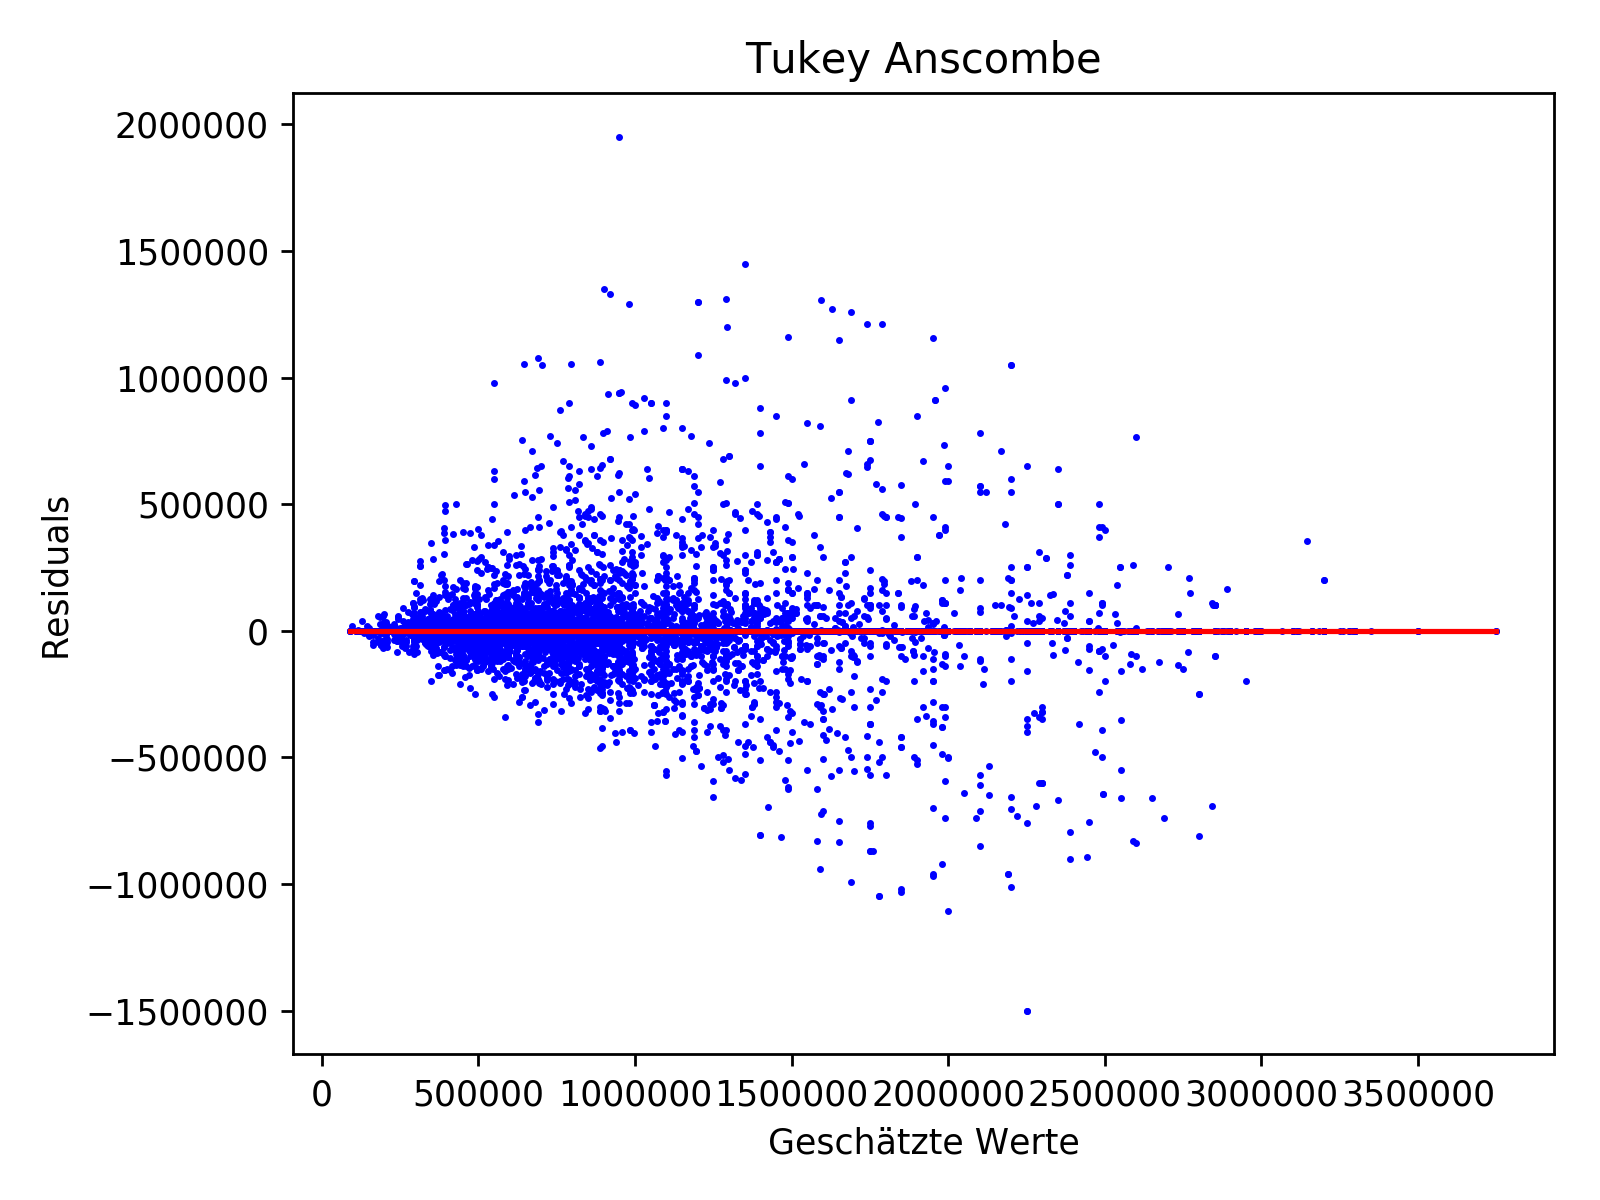
\includegraphics[width=\linewidth]{images/adaboost_tukey_anscombe_6.png}
  \caption[Tukey-Anscombe]{Tukey-Anscombe}
  \label{fig:ada_tukey-anscombe_6}
\end{subfigure}
\begin{subfigure}{.5\textwidth}
  \centering
  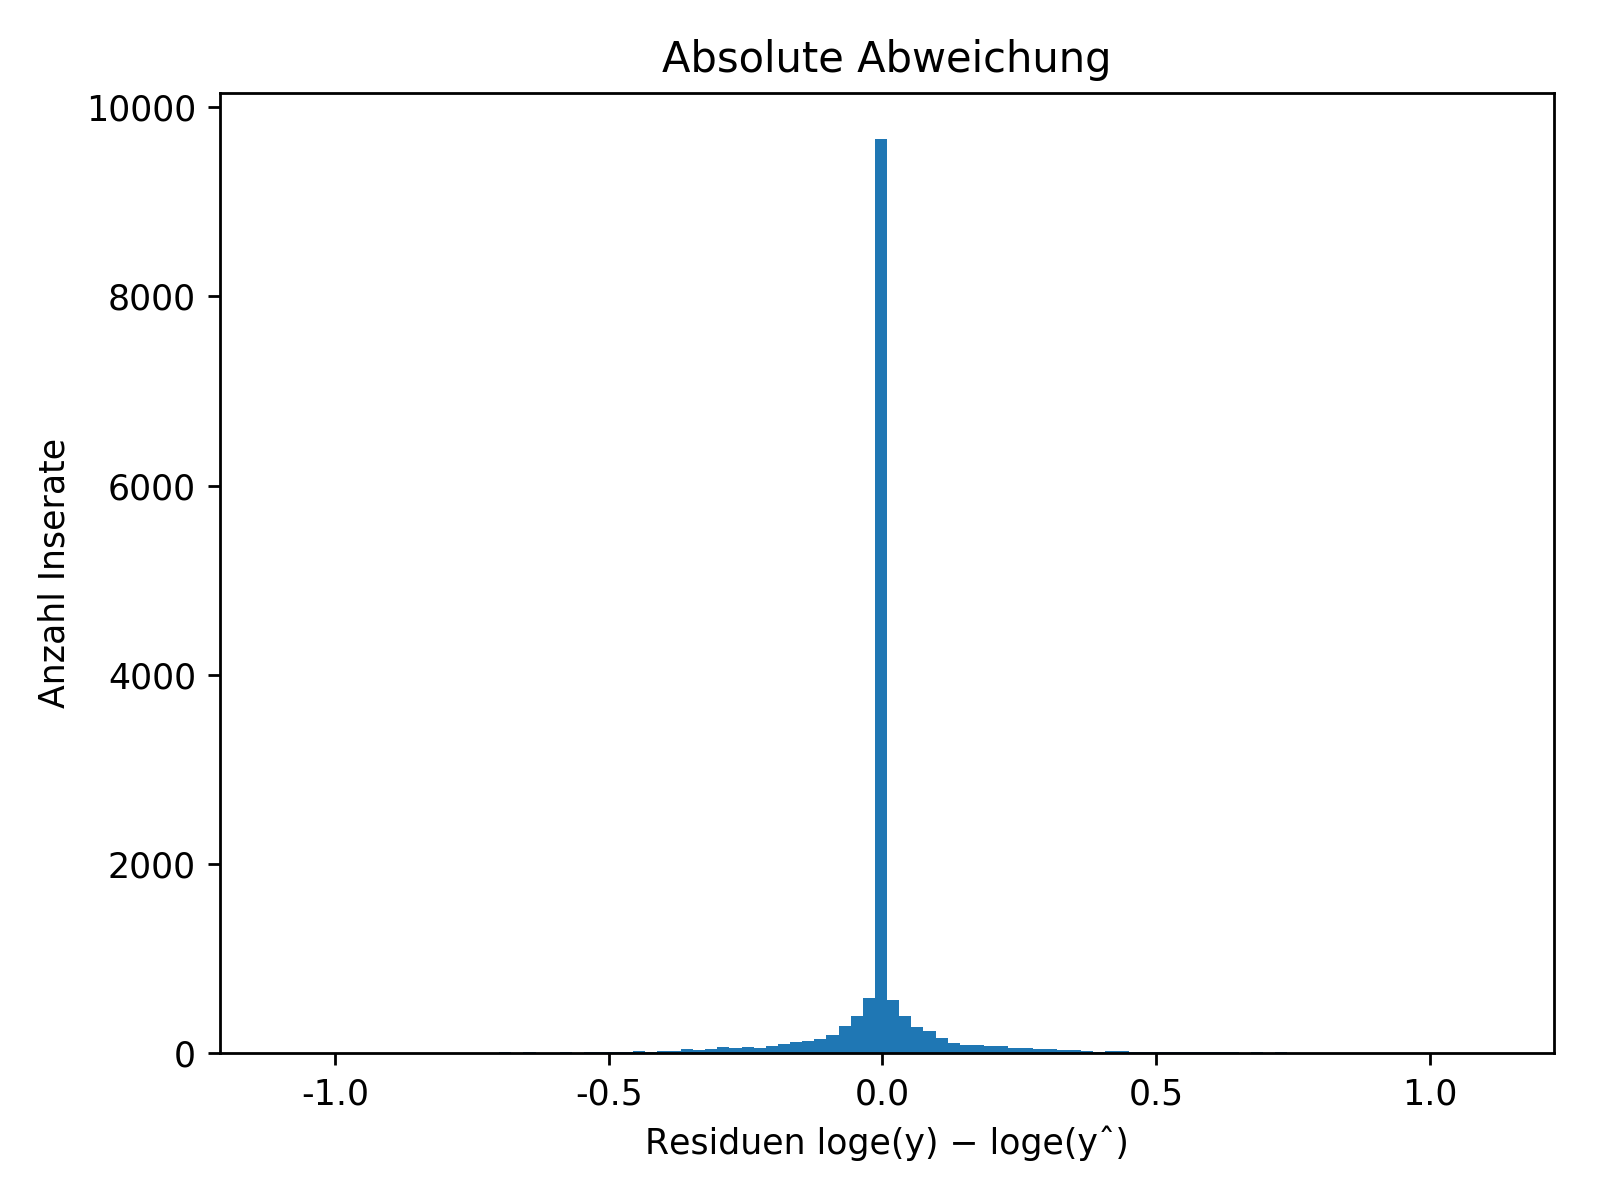
\includegraphics[width=\linewidth]{images/adaboost_verteilung_residuals_log_6.png}
  \caption[Histogramm]{Histogramm}
  \label{fig:ada_histo_6}
\end{subfigure}
\caption[Auswertung der Residuen für AdaBoost mit Outlier Detection]{Auswertung der Residuen für AdaBoost  mit Outlier Detection}
\label{fig:adaboost_6}
\end{figure}

\begin{table*}[ht]
\centering
\ra{1.3}
\resizebox{\textwidth}{!}{
\begin{tabular}{@{}lrrrrr@{}}
\toprule
Objektart & Min & Max & Durchschnitt & Median & Standardabweichung\\
\midrule
Wohnung & 90000 & 3'500'000 & 837'394 & 705'000 & 488'630\\
Haus & 125'000 & 3'750'000 & 1'082'756 & 930'000 & 541'671\\
Wohnung \& Haus & 90000 & 3'750'000 & 931'671 & 795'000 & 523'448\\
\bottomrule
\end{tabular}}
\caption{Statistische Werte des Kaufpreises nach der Outlier Detection}
\label{tab:price_outlier}
\end{table*}

\begin{table*}[ht]
\centering
\ra{1.3}
\resizebox{\textwidth}{!}{
\begin{tabular}{@{}lrrrrr@{}}
\toprule
ML Algorithmus & $R^2$ & MAPE & MdAPE & 10\% Abweichung & Maximaler Fehler\\
\midrule
Extra Trees & 0.946107 & 5.39 & 0.686 & 83.799 & 1.55E+06\\
XGBoost & 0.940157 & 5.382 & 0.632 & 83.997 & 1.82E+06\\
AdaBoost &0.943958 & 4.64 & 0 & 85.596 & 1.81e+06\\
\bottomrule
\end{tabular}}
\caption{Ergebnisse mit Einbezug des Steuerfusses}
\label{tab:sixth_round}
\end{table*}

\newpage
\clearpage
\textbf{Steuerfuss}\\
Von Interesse war, ob der Steuersatz eine Auswirkung auf das Modell besitzt. Deshalb hatten wir vom Bundesamt für Statistik den Steuerfuss für Gemeinde und Kanton beschafft. Tablle \ref{tab:sixth_round} zeigt, dass sich weder eine Verbesserung noch eine Verschlechterung mit diesen beiden Features ergab. Der Steuerfuss besass demnach keinen grossen Einfluss auf den Immobilienpreis, beziehungsweise auf die Schätzungsmodelle.

\textbf{Tag Gruppierung}\\
Unser Modell besitzt insgesamt 50 verschiedene Tags als einzelne Feature. Diese Tags hatten sich stellenweise bedeutungsmässig überschnitten. Daher lohnte es sich aus überschneidenden Features ein Feature zu bilden. Wir definierten 4 Gruppen denen wir die Tags zuordneten. 

\begin{description}
\item[Badezimmer:] Alle Tags die eine Nasszelle beschrieben. Dazu gehörte Badezimmer, Lavabo, Dusche usw.
\item[Innenausstattung:] Alle Tags die eine Innenausstattung beschrieben, wie TV Anschluss, gross, hell usw.
\item[Aussenausstattung:] In diese Kategorie fielen Tags wie Garten, Balkon, Garage, Parkplatz usw.
\item[Nachbarschaft:] Beschrieb die Umgebung der Immobilie. Ist es zentral, ruhig, hat es Einkaufsmöglichkeiten usw.
\end{description}

\begin{table*}[ht]
\centering
\ra{1.3}
\resizebox{\textwidth}{!}{
\begin{tabular}{@{}lrrrrr@{}}
\toprule
ML Algorithmus & $R^2$ & MAPE & MdAPE & 10\% Abweichung & Maximaler Fehler\\
\midrule
Extra Trees & 0.947874 & 4.854 & 0.109 & 85.541 & 2.54E+06\\
XGBoost &0.945822 & 4.881 & 0.074 & 85.759 & 2.50E+06\\
AdaBoost &0.93973 & 4.544 & 0 & 86.317 & 2.60E+06\\
\bottomrule
\end{tabular}}
\caption{Ergebnisse mit gruppierten Tags}
\label{tab:seventh_round}
\end{table*}

Die Ergebnisse in Tabelle \ref{tab:seventh_round} zeigen nochmals eine kleine Verbesserung der Performance. In Abbildung \ref{fig:adaboost_8} ist ersichtlich, dass die geschätzten Werte nochmal ein Stück näher am Beobachtungswert liegen.

\begin{figure}[h]
\begin{subfigure}{.5\textwidth}
  \centering
  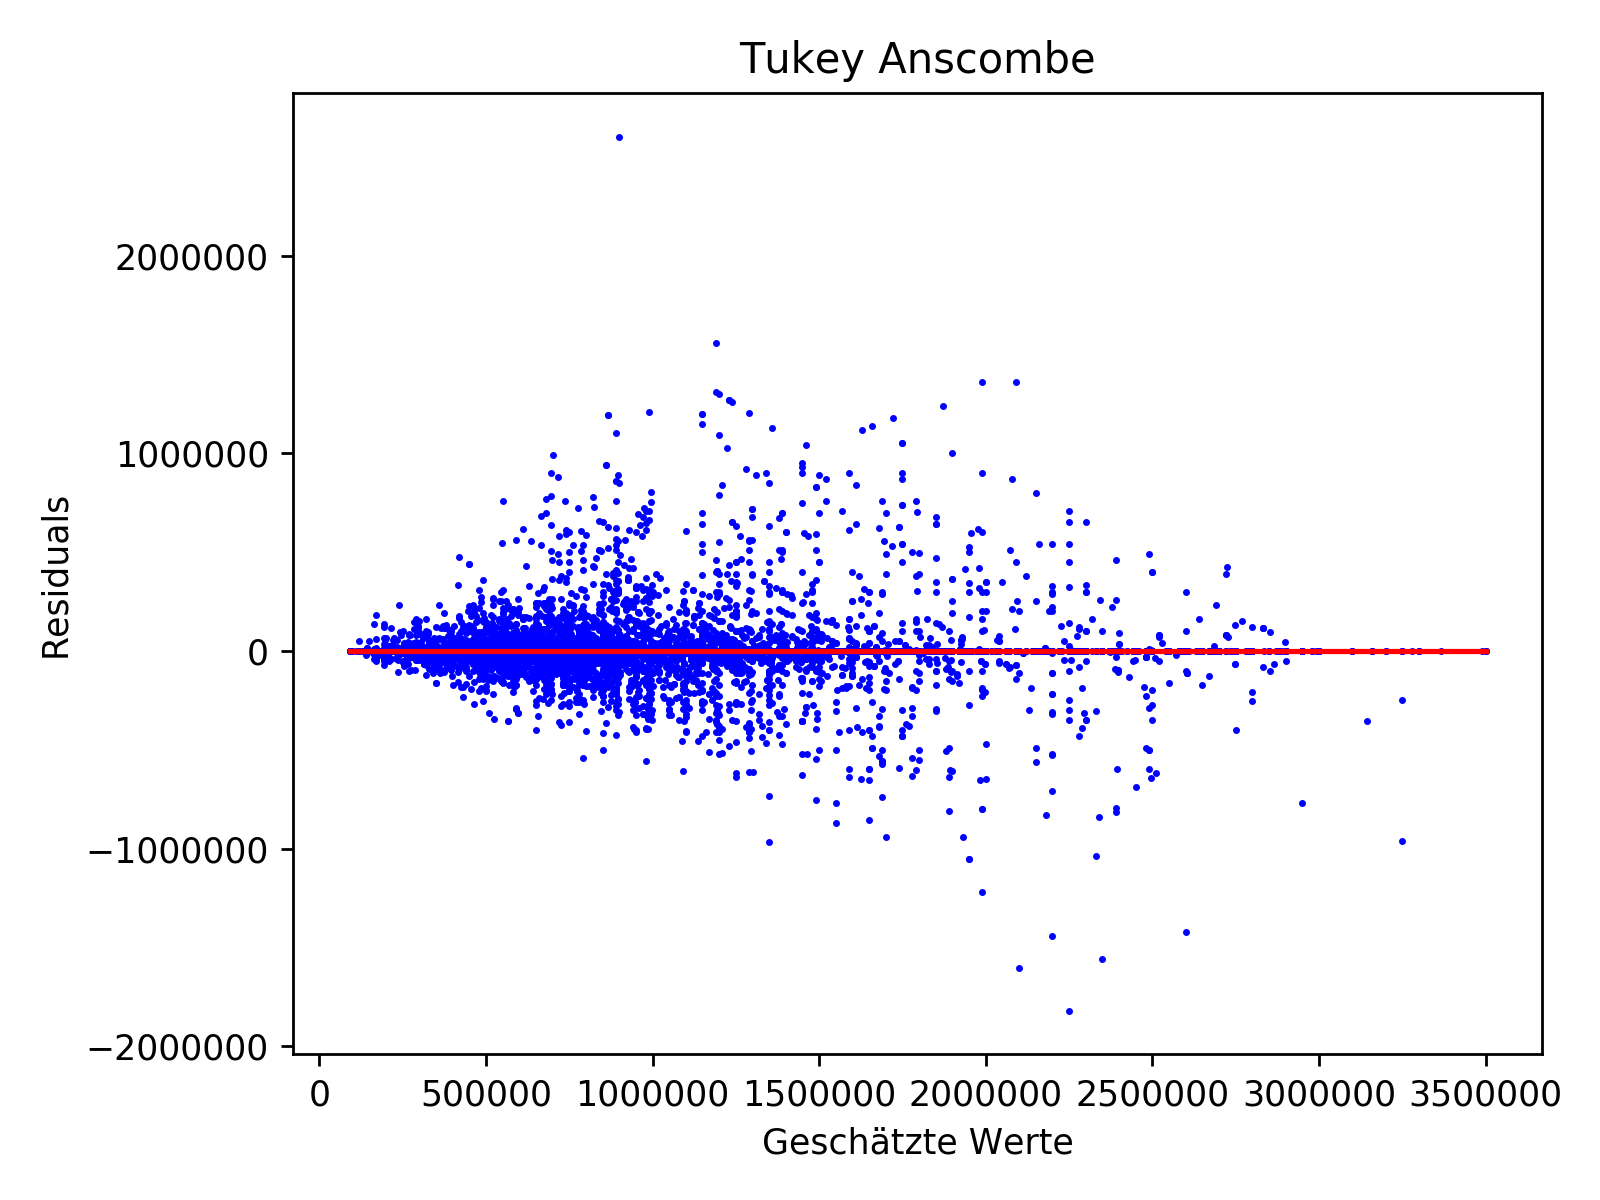
\includegraphics[width=\linewidth]{images/adaboost_tukey_anscombe_8.png}
  \caption[Tukey-Anscombe]{Tukey-Anscombe}
  \label{fig:ada_tukey-anscombe_8}
\end{subfigure}
\begin{subfigure}{.5\textwidth}
  \centering
  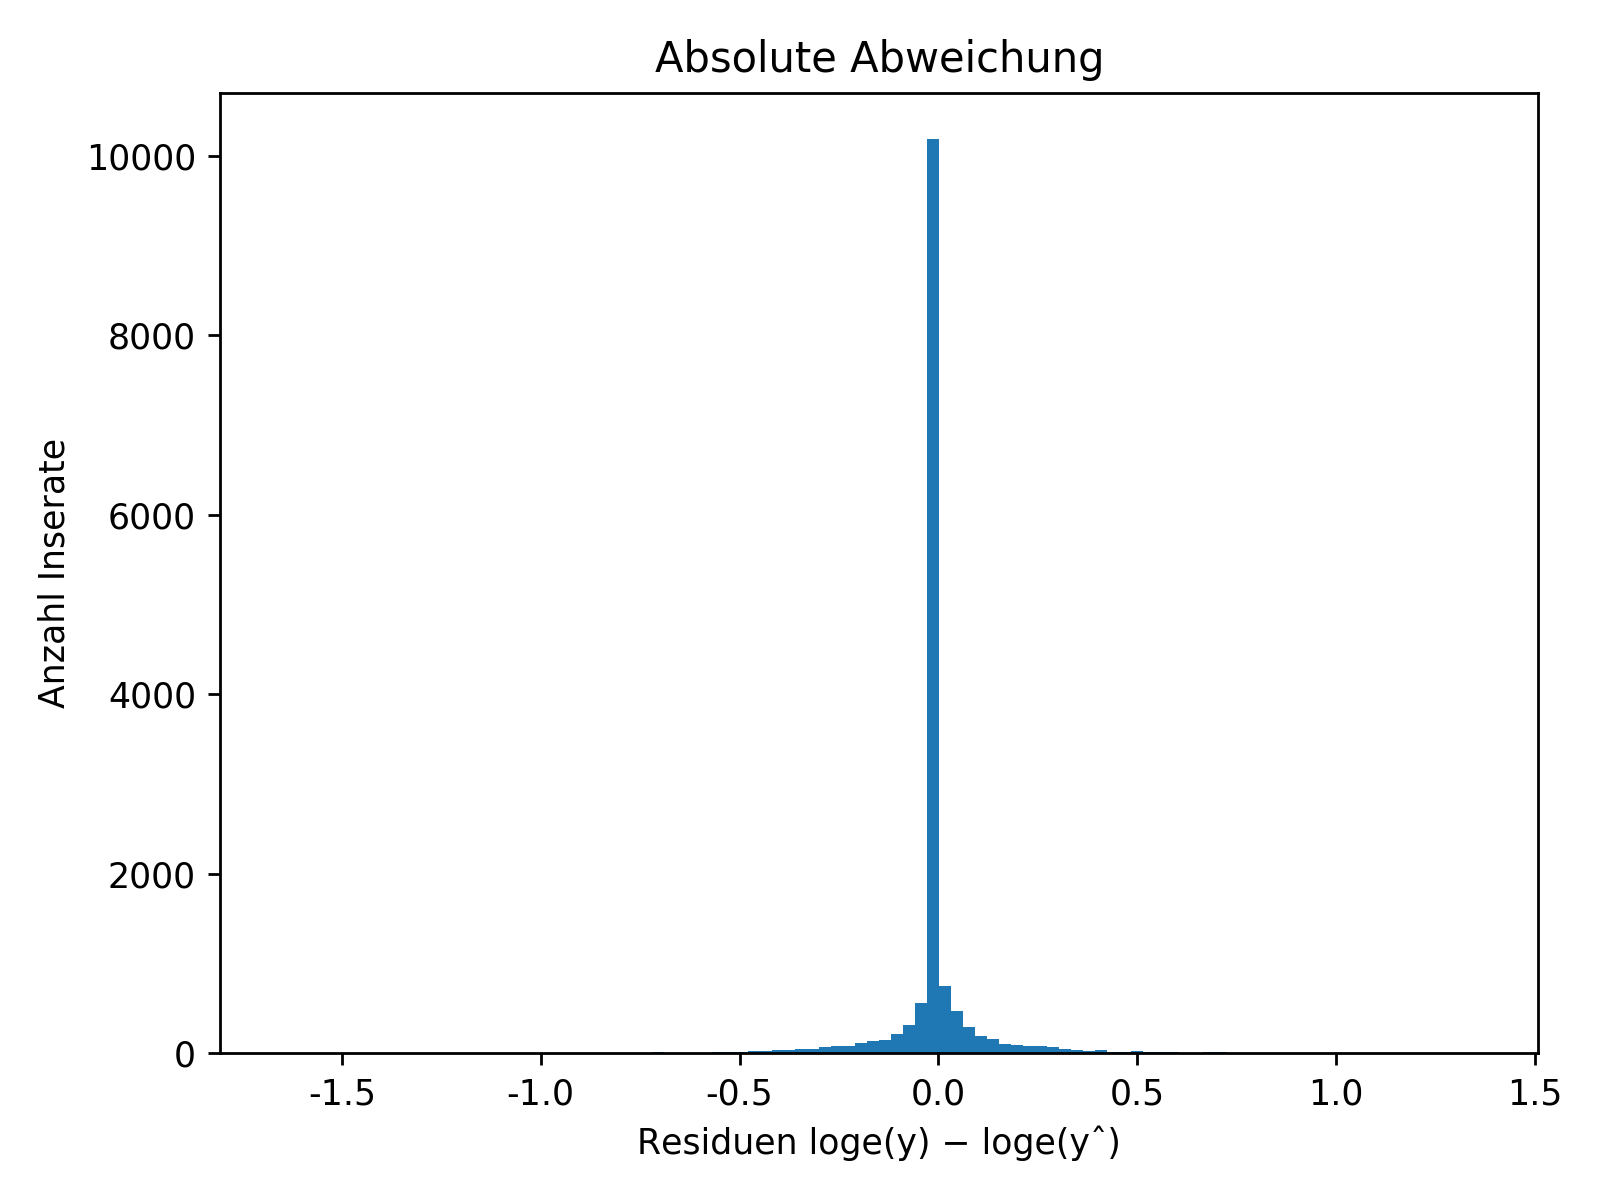
\includegraphics[width=\linewidth]{images/adaboost_verteilung_residuals_log_8.png}
  \caption[Histogramm]{Histogramm}
  \label{fig:ada_histo_8}
\end{subfigure}
\caption[Auswertung der Residuen für AdaBoost mit komplettem Feature Engineering]{Auswertung der Residuen für AdaBoost mit komplettem Feature Engineering}
\label{fig:adaboost_8}
\end{figure}

\begin{table*}[ht]
\centering
\ra{1.3}
\resizebox{\textwidth}{!}{
\begin{tabular}{@{}lrrrrr@{}}
\toprule
ML Algorithmus & $R^2$ & MAPE & MdAPE & 10\% Abweichung & Maximaler Fehler\\
\midrule
Extra Trees & 0.907327 & 7.092 & 0.684 & 79.063 & 1.96E+06\\
XGBoost & 0.892067 & 8.692 & 0.941 & 78.207 & 2.16E+06\\
AdaBoost & 0.893971 & 7.054 & 0 & 80.176 & 1.96E+06\\
\bottomrule
\end{tabular}}
\caption{Ergebnisse ohne ortsbezogenen Daten vom BFS}
\label{tab:height_round}
\end{table*}

\textbf{Ohne ortsbezogene Daten}\\
Mit unserem Feature Engineering konnten wir aufzeigen, dass eine deutliche Verbesserung der Modelle erreicht werden konnte. Für die Forschungsfrage, \textit{Wie stark kann das Resultat verbessert werden, wenn geobasierte Daten hinzugefügt werden?}, untersuchten wir die Resultate ohne Daten vom BFS. Es ist in Tabelle \ref{tab:height_round} gut ersichtlich, dass ohne ortsbezogene Daten ein schlechteres Modell berechnet wurde.

\subsubsection{Kombinierte Algorithmen}
Als weiteren Test haben wir einen eigenen Regressor erstellt, der mehrere Machine Learning Algorithmen kombiniert.

Dieser Algorithmus hatte im Endeffekt zwei Schätzphasen. Zunächst wurde ein Extra Trees trainiert und für jeden Trainingsdatensatz wurden alle Entscheidungspfade für alle Bäume abgespeichert. Um nun eine Schätzung zu erhalten, wurden zuerst die Entscheidungspfade für den zu testenden Datensatz herausgesucht, und mit den Trainingsdatensatz verglichen. Alle Trainingsdatensätze mit mindestens einem passendem Entscheidungspfad wurden markiert für die zweite Phase der Schätzung.\\
In der zweiten Phase wurden diese markierten Datensätze auf einem weiteren Machine Learning Algorithmus ad-hoc trainiert. Der zweite Algorithmus konnte nach belieben ausgetauscht werden. Anschliessend wurde auf diesem neuen Modell der Testdatensatz geschätzt.\\
Theoretisch wäre es möglich gewesen, für alle möglichen Entscheidungspfade die Modelle im Vorhinein zu berechnen, da nur eine finite Anzahl an Entscheidungspfade existierten. Dies war aber aus praktikablen Gründen nicht möglich, da mit vielen Datensätzen die trainierten Bäume gross wurden und entsprechend dafür zu viel RAM und Rechenzeit benötigt wurde.

Um genügend Datensätze für die zweite Phase zu erhalten, wurde der Extra Trees mit einer minimalen Leaf Size von fünf Samples konfiguriert.\\
Für den zweiten Schätzungsalgorithmus verwendeten wir den $K$-Nearest Neighbor wie oben im Kaptiel \ref{chapter:KNN} beschrieben. Wie in Tabelle \ref{tab:combined} erkennbar, waren die Ergebnisse weitaus schlechter als oben verwendete Algorithmen.

\begin{table*}[ht]
\centering
\ra{1.3}
\resizebox{\textwidth}{!}{
\begin{tabular}{@{}lrrrrr@{}}
\toprule
ML Algorithmus & $R^2$ & MAPE & MdAPE & 10\% Abweichung & Maximaler Fehler\\
\midrule
Extra Trees mit KNN & 43.636 & 13.451 & 40.034 &  0.619114 & 2.94294e+07\\
\bottomrule
\end{tabular}}
\caption{Ergebnisse des selbst entwickelten Algorithmus}
\label{tab:combined}
\end{table*}

Als letztes kombinierten wir noch die drei Baumalgorithmen miteinander. Verschiedene Tests zeigten, dass die Gewichtung von 70\% AdaBoost, 20\% XGBoost und 10\% Extra Trees die beste Performance lieferten.
Das Resultat in Tabelle \ref{tab:combined_2} zeigt die Performancewerte.

\begin{table*}[ht]
\centering
\ra{1.3}
\resizebox{\textwidth}{!}{
\begin{tabular}{@{}lrrrrr@{}}
\toprule
ML Algorithmus & $R^2$ & MAPE & MdAPE & 10\% Abweichung & Maximaler Fehler\\
\midrule
Kombiniert & 0.94646 & 4.416 & 0.07 & 87.03	& 1.77E+06\\
\bottomrule
\end{tabular}}
\caption{Kombination von AdaBoost, XGBoost und Extra Trees}
\label{tab:combined_2}
\end{table*}

\subsection{Auswertung}
Es hat sich gezeigt, dass eine Kombination von AdaBoost, Extra Trees und XGBoost die besten Resultate erzielt (siehe Tabelle \ref{tab:combined_2}). Werden die Algorithmen alleine betrachtet, hatte bei unseren Daten der AdaBoost die besten Ergebnisse erreicht.\\
Von der Berechnungszeit ist AdaBoost klar der beste Algorithmus, da dieser für einen Fit ungefähr 10 Minuten benötigte, während XGBoost und Extra Trees über eine Stunde brauchten.

Wir konnten mit unserer eigenen Implementation eines Machine Learning Algorithmus keinen Erfolg erzielen, da die Performance nicht zufriedenstellend war. Bei den linearen Regressionsalgorithmen konnte auch keine akzeptable Performance erreicht werden. Der Grund dafür liegt bei den vielen kategorischen Features. Der $K$-Nearest Neighbor ist zwar viel besser als die linearen Regressionen, aber kommt nicht an die Ergebnisse der Baumalgorithmen an.

Weiter konnte bewiesen werden, dass ortsbezogene Daten das Resultat masgeblich verbessern konnten. In unserem Fall büsste die MAPE 2.5\% ein und es konnten 7\% weniger Häuser mit einer maximalen Abweichung von 10\% richtig geschätzt werden. So konnte aufgezeigt werden, dass bei einer Schätzung eines Immobilienpreises, der Standort mit seinen Eigenschaften für das Schätzungsmodell wichtig war.\\[2ex]
%
Die Qualität der Daten von Immobilienplattformen war eher durchmischt. Es existierten qualitativ sehr gute Inserate, mit vielen Kennwerten und einer ausführlichen Beschreibung. Im Schnitt jedoch konnten neben dem Preis nur die vier Kennwerte Wohnfläche, Anzahl Zimmer, Baujahr und Renovationsjahr verwendet werden.\\
Mit einem ausgiebigen Feature Engineering und einer genügenden Menge an Inseraten, fielen die qualitativ schlechten Inserate weniger ins Gewicht, beziehungsweise wurden aussortiert.  So konnten von insgesamt 162’225 Inseraten 85’845 für den Machine Learning Teil aufbereitet werden. Dies entspricht 52\% der Inserate.\\
Die Outlier Detection spielte dabei eine wichtige Rolle, da sie den maximalen Fehler stark reduzierte, indem sie 12'362 abnormale Inserate entfernte. Zudem reduzierte sie die Standardabweichung um mehr als die Hälfte.

Beim Crawlen zeigte sich, dass es sich lohnte über mehrere Proxyinstanzen zu gehen, um eine Sperrung zu verhindern. Die Inserate konnten weitgehend ohne Probleme gesammelt und aufbereitet werden.
%
\subsection{Gültigkeitsrisiken}
Zu beachten gilt, dass wir unsere Modelle auf geschätzten Werten trainiert haben. Somit sind unsere Schätzungen als Unterstützung und nicht als Endpreis zu betrachten. Zudem ist der Immobilienpreis immer gewissen Schwankungen ausgesetzt. Die Modelle schätzen somit die Immobilienpreise in der gesammelten Zeit. Für eine spätere Evaluation müsste ein neues Datenset mit aktualisierten Immobilienpreisen verwendet werden.\\
Ein Blick auf die Verteilung des Preises zeigt, dass sich der Preis primär zwischen 250'000 CHF und 1.2~Mio,~CHF befindet. Dadurch können extraordinäre, sowie günstige  Immobilien nur sehr schwer geschätzt werden.\\[2ex]
%
Wir haben die Kennwerte von öffentlichen Immobilienplattformen gesammelt. Dort geht es hauptsächlich darum, die Immobilie zu verkaufen. So wird gerne bei den Kennwerten geschummelt, oder schöngeredet indem sie falsch eingetragen werden. Eine Outlier Detection kann nur grobe Ausreisser erkennen, kleinere Ausreisser bleiben somit unentdeckt und verfälschen das Modell.\\
Wird eine neue Siedlung oder ein neuer Wohnblock inseriert, kann es vorkommen, dass 10 mal die gleiche Wohnung inseriert wird. Dies ist unschön, da diese Wohnungen im Modell mehr Gewicht erhalten. Wir haben uns jedoch stark bemüht, solche Duplikate zu erkennen und zu entfernen.

%1970 von ingesamt 73483